%\section{Results}
Thus far I have outlined all reconstruction-level inputs to our analysis including event selection, backgrounds and their estimation methods, and systematic uncertainties. Each of these components is critical to our final result. This section will focus on the methods used to extract the VBF $H\rightarrow WW^*$ cross-section measurement. 
\section{Statistical analysis}
\subsection{Likelihood functions}
This analysis rests on the estimation of a parameter $\mu$, signal strength, which describes the statistical significance of our signal yield relative to its Standard Model prediction and, in this particular analysis, defines the signal cross-section and signal and background yields. 

We build a likelihood function, $\mathcal{L}(\mu,\Theta)$, where the signal strength $\mu$ is a parameter of interest (POI) and nuisance parameters (NPs) $\Theta=\Theta_a,\Theta_b,...$ represent all relevant uncertainties. None of these values are known \textit{a priori}, so the likelihood is built to represent the probability of particular values for the POIs and NPs. The analysis uses a maximum likelihood estimator to find the inputs which maximize the likelihood, i.e. minimize the negative log of the likelihood. Here I will briefly outline how a likelihood function can incorporate regions of interest. This discussion uses Ref.~\cite{cranmer2015practical} as a guide. The Poisson distribution $\mathcal{P}(n|\lambda)$ describes the probability of $n$ events with a true unknown yield $\lambda$:
\begin{equation}
\mathcal{P}(n|\lambda)= \lambda^n\frac{e^{-\lambda}}{n!}.
\end{equation}
We can define a variable observable $x$ with probability density $f(x)$, hence with $n$ events the probability density of each is multiplied. The likelihood of $\lambda$ can now be written as
\begin{equation}
\mathcal{L}(\lambda)=\mathcal{P}(n|\lambda)\prod_{\text{event}}^n f(x).
\end{equation}
Our likelihood also must take into account multiple regions (the signal region as well as the control regions) and these likelihoods are multiplied together with their own distinct Poisson distributions,
\begin{equation}
\mathcal{L}(\lambda)=\prod_r^{\text{regions}}(\mathcal{P}(n_r|\lambda_r)\prod_{\text{event}}^n f(x)).
\end{equation}
Our statistical fit maximizes this likelihood function and so produces a yield $\lambda$ for each free parameter simultaneously. The $\lambda$ values represent predicted yields where $\lambda_{r,b} = \mu \lambda_{\text{sig}}+\lambda_{\text{bkg}}$. Maximizing the overall likelihood is made simpler by applying the natural logarithm, as the products between Poisson distributions become summations.  

Particle physics defines discovery with rigorous standards using hypothesis testing. In the fit, we consider both the null (background-only) hypothesis, in which $\mu=0$, and the alternative hypothesis, in which we consider both signal and background to be present. The probability that the null hypothesis is rejected (or that the signal is discovered) is defined using a $p$-value. The $p$-value can be converted to a number of Gaussian standard deviations. In high-energy physics a 3 $\sigma$ significance, $p$-value of $1.35 \times 10^{-3}$, is considered evidence, while a 5 $\sigma$ result, $p$-value $2.87\times10^{-7}$, is considered a discovery.

This analysis uses the HistFitter software compiled with RooStats, RooFit, and HistFactory to perform the likelihood maximization. We measure the signal VBF Higgs cross-section in the fiducial space defined by the signal region selection with a simultaneous fit to the signal and control regions. Each region has a different distribution used in the fit to maximize that discrimination of each respective sample against all other events. This fit includes as floating parameters the signal strength of seven different processes: $\mu_{VBF}$, $\mu_{TopWW}$, $\mu_{Z+jets}$, $\mu_{ggFSR}$, $\mu_{ggF1}$, $\mu_{ggF2}$, and $\mu_{ggF3}$. Each numbered ggF parameter is estimated in an orthogonal control region described in Chapter 6 while ggF SR is measured in the signal region with a targed discriminant to differentiate VBF and ggF events. Other backgrounds, mis-identified leptons, $V/\gamma$, $VH$, and $ttH$, are included as fixed parameters. 

The background treatment differs depending on the particular region and sample. For $Z+$jets, a designated control region is used and the yield in the signal region is found by including a transfer factor, which maps the yield in the $Z+$jets control region to that in the signal region. Transfer factors to extrapolate yields are derived by normalizing to MC simulation. For backgrounds estimated within the signal region (Top/$WW$) the transfer factor is used only to extrapolate into the control regions where the contribution enters and thus uncertainties associated with transfer factors are reduced. We use the predicted MC values for all backgrounds included as fixed parameters such as $V\gamma$, $VH$, and $ttH$. We use a data-driven method to estimate the mis-identified lepton background. 

Events in the $e\mu$ and $\mu e$ channels are combined in the analysis and the likelihood is defined as the product of the Poissonians over BDT output bins in the signal region multiplied by the product of Poissonians over discriminant distributions in the controls regions (ggF CRs, $Z+$jets CR and Top/WW CR- within the signal region). The likelihood can then be calculated 

\begin{equation}
  \begin{aligned}
\mathcal{L}(\mu) = \displaystyle\prod_{j=0}^{N_{\text{sig BDT bins}}} \mathcal{P} (n_{j}|\lambda_r) \times \displaystyle\prod_{k=1}^{N_{\text{CR-bins}}} P(n_{k}|\lambda_b) \\
\qquad = \displaystyle\prod_{j=0}^{N_{\text{sig BDT bins}}} \mathcal{P} (n_{j}|\mu_s \lambda_{sig,j} + \displaystyle\sum_{n}^{N_{\text{bkg}}}\mu_b^{n} \lambda_{bkg}^{nj}) \times \displaystyle\prod_{k=1}^{N_{\text{CR-bins}}} P(n_{k}|\mu_s \lambda_{sig,k} + \displaystyle\sum_{n}^{N_{\text{bkg}}}\mu_b^{n} \lambda_{bkg}^{nk}).
  \end{aligned}
\end{equation}

The signal and background strengths are denoted $\mu$ and the yields $\lambda$. Sums over all $n$ backgrounds include $Z+$jets, top/$WW$, and ggF; the minor backgrounds and data-driven $W+$jets estimate are added to Poisson expectations as fixed parameters. 

The last important additions to this likelihood are nuisance parameters. These parameters, $\Theta$, come in two general types: systematics which do not affect the shape of discriminating variables ("flat systematics") and those that do ("shape systematics"). Flat systematics are constrained with a unit Gaussian and their effects are measured for $\Theta=\pm1$. Shape systematics are constrained with a unit Gaussian as well though their effects are measured through $\nu_{\text{shape}}(\Theta)= 1+\epsilon\Theta$, where $\epsilon$ is determined by measuring $\nu_{\text{shape}}$ at $\Theta=\pm 1$. Adding nuisance parameters $\Theta$ our final likelihood can be written 
\begin{equation}
  \begin{aligned}
\mathcal{L}(\mu,\vec{\Theta}) = \displaystyle\prod_{j=0}^{N_{\text{sig BDT bins}}} \mathcal{P} (n_{j}|\mu_s \lambda_{sig,j} + \displaystyle\sum_{n}^{N_{\text{bkg}}}\mu_b^{n} \lambda_{bkg}^{nj}) \times \displaystyle\prod_{k=1}^{N_{\text{CR-bins}}} P(n_{k}|\mu_s \lambda_{sig,k} + \displaystyle\sum_{n}^{N_{\text{bkg}}}\mu_b^{n} \lambda_{bkg}^{nk})  \times
  \displaystyle\prod_{i=1}^{N_{\Theta_i}}G(\tilde{\Theta_i}|\Theta_i,1)
  \end{aligned}
\end{equation}
where $G(\tilde{\Theta_i}|\Theta_i,1) = \frac{1}{\sqrt{2\pi}}e^{\frac{(\tilde{\Theta}-\Theta)^2}{2}}$ is the unit Gaussian and $\tilde{\Theta}$ is an auxiliary measurement of $\Theta$.

The fit is performed simultaneously for the signal region, three ggF control regions, a $Z+$jets control region, and a shared top/$WW$ control defined within the signal region. Table~\ref{tab:regiondefinitions} summarizes the regions used within the fit and their defining selections. These are discussed in more detail in Chapters 5 and 6. 

\begin{table}[h!]
\begin{center}
\resizebox{\textwidth}{!}{
\begin{tabular}{|c|c|c|c|c|c|c|}
\hline
\textbf{Signal region}   & \textbf{Top/$WW$ CR} & \textbf{$Z+$jets CR} & \textbf{ggF SR} & \textbf{ggF CR1} & \textbf{ggF CR2} & \textbf{ggF CR3} \\
\hline
\hline
\multicolumn{6}{|c|}{$n_{jets} \geq 2$}   & $n_{jets} <2$ \\
\hline
\multicolumn{7}{|c|}{b-veto} \\
\hline
\multicolumn{4}{|c|}{CJV} & CJV/!OLV \textbar\textbar !CJV/OLV & !CJV & - \\
\hline
\multicolumn{4}{|c|}{OLV} & - & !OLV & - \\
\hline
\multicolumn{2}{|c|}{$Z$-veto} & $m_{\tau\tau}$ &\multicolumn{4}{|c|}{$Z$ veto} \\
\hline
\multicolumn{2}{|c|}{$m_{jj}>200$ GeV} & $m_{\ell\ell}<80$ GeV & \multicolumn{4}{|c|}{$m_{jj}>200$ GeV} \\
\hline
\multicolumn{2}{|c|}{$\Delta Y_{jj}>2.1$}     & - & \multicolumn{4}{|c|}{$\Delta Y_{jj}>2.1$} \\
\hline
BDT$_{\text{VBF}} \geq 0$  & BDT$_{\text{VBF}} < 0$ & -& -0.5$<$BDT$_{\text{VBF}}<0$ & -  & -  & - \\
\hline
\end{tabular}}
\end{center}
\caption{Summary of all signal and control regions included in simultaneous fit}
\label{tab:regiondefinitions}
\end{table}

Each of the regions included in the fit uses a different discriminant to best characterize that sample's contribution. These discriminants are almost all BDT outputs trained on various kinematic distributions to characterize certain background and signal samples, as discussed in Chapters 5 and 6. The $Z+$jets control region is defined with $m_T$ instead of a designated BDT after studies showed its success at mitigating uncertainty on $\mu_{Z+\text{jets}}$. These studies are included in Appendix B. Table~\ref{tab:fitinputs} summarizes the fit regions and shows their discriminant and number of bins. Table~\ref{tab:cryields} shows MC event yields in all regions included in the statistical analysis. 
\begin{table}[!h]
  \begin{center}
   \resizebox{\textwidth}{!}{
    \begin{tabular}{l|ccccccc}
       Category		& SR 	& Top/$WW$ CR 	& $Z+$jets CR 	& ggF-SR & ggF-CR1 		& ggF-CR2 	& ggF-CR3 \\
      \hline
      Discriminant	& BDT$_{\text{VBF}}$ &  BDT$_{\text{TopWW}}$	& $m_{\text{T}}$ & BDT$_{\text{ggFVBF}}$ & BDT$_{\text{ggF1}}$	& BDT$_{\text{ggF2}}$ & BDT$_{\text{ggF1}}$ \\
      Number of bins    &  25 	      & 8 	& 20 		& 25	& 8 			& 8 		& 8  \\	
    \end{tabular}}
    \caption{Fit categories, including SR and CRs, distributions and number of bins used in the fit.}
    \label{tab:fitinputs}
  \end{center}
\end{table}

\begin{table}[!h]
  \begin{center}
    \begin{tabular}{l|cccccc}
      Category         & SR    & Top/$WW$ CR   & $Z+$jets CR           & ggF-CR1               & ggF-CR2       & ggF-CR3 \\
      \hline
      \hline
      VBF      & 149.7 & 14.1 & 16.1 & 100.4 & 8.6 & 192.3 \\
      Top    &  385.9 & 2878.7 & 331.3 & 34110.4 & 10546.4 & 40206.3 \\
      $WW$ & 202.0 & 969.0 & 122.6 & 9653.7 & 2608.5 & 86387.7 \\
      ggF & 72.4 & 30.3 & 11.7 & 543.1 & 114.1 & 4069.1 \\
      $Z+$jets & 313.1 & 476.4 & 1391.1 & 5288.5 & 1395.6 & 131014.0 \\
      Fakes & 63.5 & 123.4 & 16.7 & 1752.9 & 570.0 & 15166.2 \\
      $V\gamma$ & 23.5 & 33.7 & 36.7 & 490.7 & 94.9 & 4652.9 \\
      $VH$ & 2.0 & 2.4 & 1.4 & 89.7 & 18.5 & 164.6 \\
      $ttH$ &  3.8 &  5.9 &  19.8 & 35.5 & 8.5 & 437.6 \\
      \hline
    \end{tabular}
    \caption{MC event yields in each signal and control region pre-fit.}
    \label{tab:cryields}
  \end{center}
\end{table}

\subsection{Asimov results}
The Asimov dataset is formed with Monte Carlo pseudo-experiments and by design returns the true value for each estimated parameter. We use the Asimov dataset to test analysis strategies and deduce expected performance of the fit without using true data. We ``blind'' the data by removing events in the uppermost bins of the BDT$_{\text{VBF}}$ distribution and use only Monte Carlo events in the signal region to eliminate any potential bias. Using this approach, we gain an understanding for the constraints on our nuisance parameters and their expected uncertainties. Using the Asimov dataset, all floating parameters are measured to be 1 and all nuisance parameters 0. Results of the fitted nuisance parameters to the Asimov dataset are made under the hypothesis that VBF Higgs boson cross-sections follow our Standard Model predictions. 

Fit results for each of the signal strength parameters in our statistical fit are calculated with statistical uncertainties only and statistical$+$systematic uncertainties. The results for statistical uncertainties are calculated by fixing each nuisance parameter to the value determined by the full systematic fit. We can similarly determine the effect of all theoretical and experimental uncertainties by fixing all but the tested systematics and then subtracting the statistical contribution in quadrature. After including all uncertainties and performing a one dimensional scan of $\mu_\text{VBF}$, the Asimov dataset provides an expected precision of ($^{+21.0\%}_{-18.8\%}$) on $\mu_{VBF}$. This is broken down into components:
\begin{equation}
\mu_{\text{exp}} = 1.000 ^{+0.21}_{-0.19} \text{ (Total) } ^{+0.17}_{-0.16} \text{ (Stat.) } ^{+0.11}_{-0.08} \text{ (Theor.) } ^{+0.05}_{-0.05} \text{ (Exp.) }.
\end{equation}

This corresponds to an expected null $p$-value of $2.7\times10^{-10}$ or a signficance of 6.2$\sigma$, which is more than twice the expected significance in the last published ATLAS VBF Higgs $\rightarrow \ell\nu\ell\nu$ result ~\cite{Aaboud_2019}.   
%The expected and observed yields in the signal region are shown in Table~\ref{tab:sryields} and lead to the final cross section measurement.  

%\begin{table}[!h]
%  \begin{center}
%    \begin{tabular}{l|c|c|}
%	& \multicolumn{2}{|c|}{Estimated Uncertainty}\\
%       \hline
%        Parameter & Stat-only    & Stat + Sys \\
%      \hline
%       $\mu_{\text{VBF}}$ & 15.7 $\%$ & 18.2$\%$ \\
%       $\mu_{\text{top/}WW}$ & 0.5 $\%$ & 15.3$\%$\\
%       $\mu_{\text{ggF-SR}}$ & 159.0 $\%$ & 134.0$\%$ \\
%       $\mu_{\text{ggF1}}$ & 20.8 $\%$ & 24.7$\%$ \\
%       $\mu_{\text{ggF2}}$ & 47.3 $\%$ & 51.6$\%$ \\
%       $\mu_{\text{ggF3}}$ & 21.6 $\%$ & 25.5$\%$ \\
%       $\mu_{Z+\text{jets}}$ & 2.1 $\%$ & 18.6$\%$ \\
%    \end{tabular}
%    \caption{Asimov fit results for all floating parameters in stat-only and full systematic fits.}.
%    \label{tab:muresults}
%  \end{center}
%\end{table}

\begin{figure}[!h]
\centering
%  \subfloat[$\mu_{\text{VBF}}$]{
      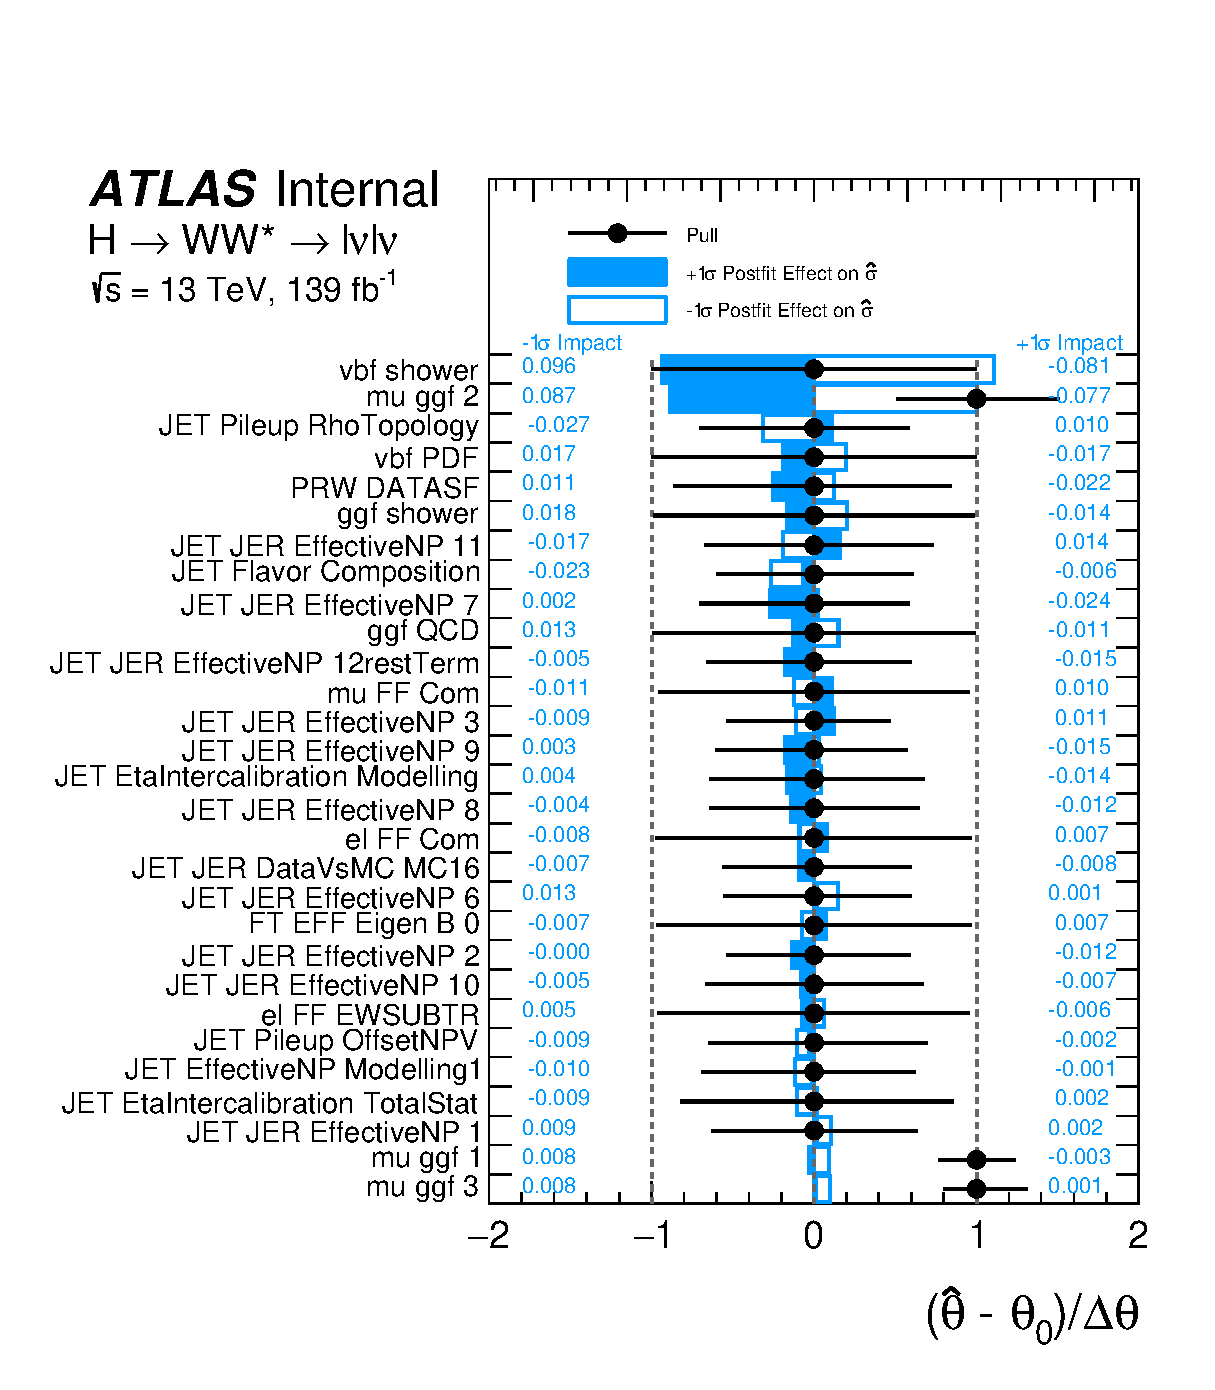
\includegraphics[width=0.6\textwidth]{Pictures/fitresults/impact_asimov_mu_vbf.eps}
%  }\hfill
%  \subfloat[$\mu_{\text{ggF}}$]{
%      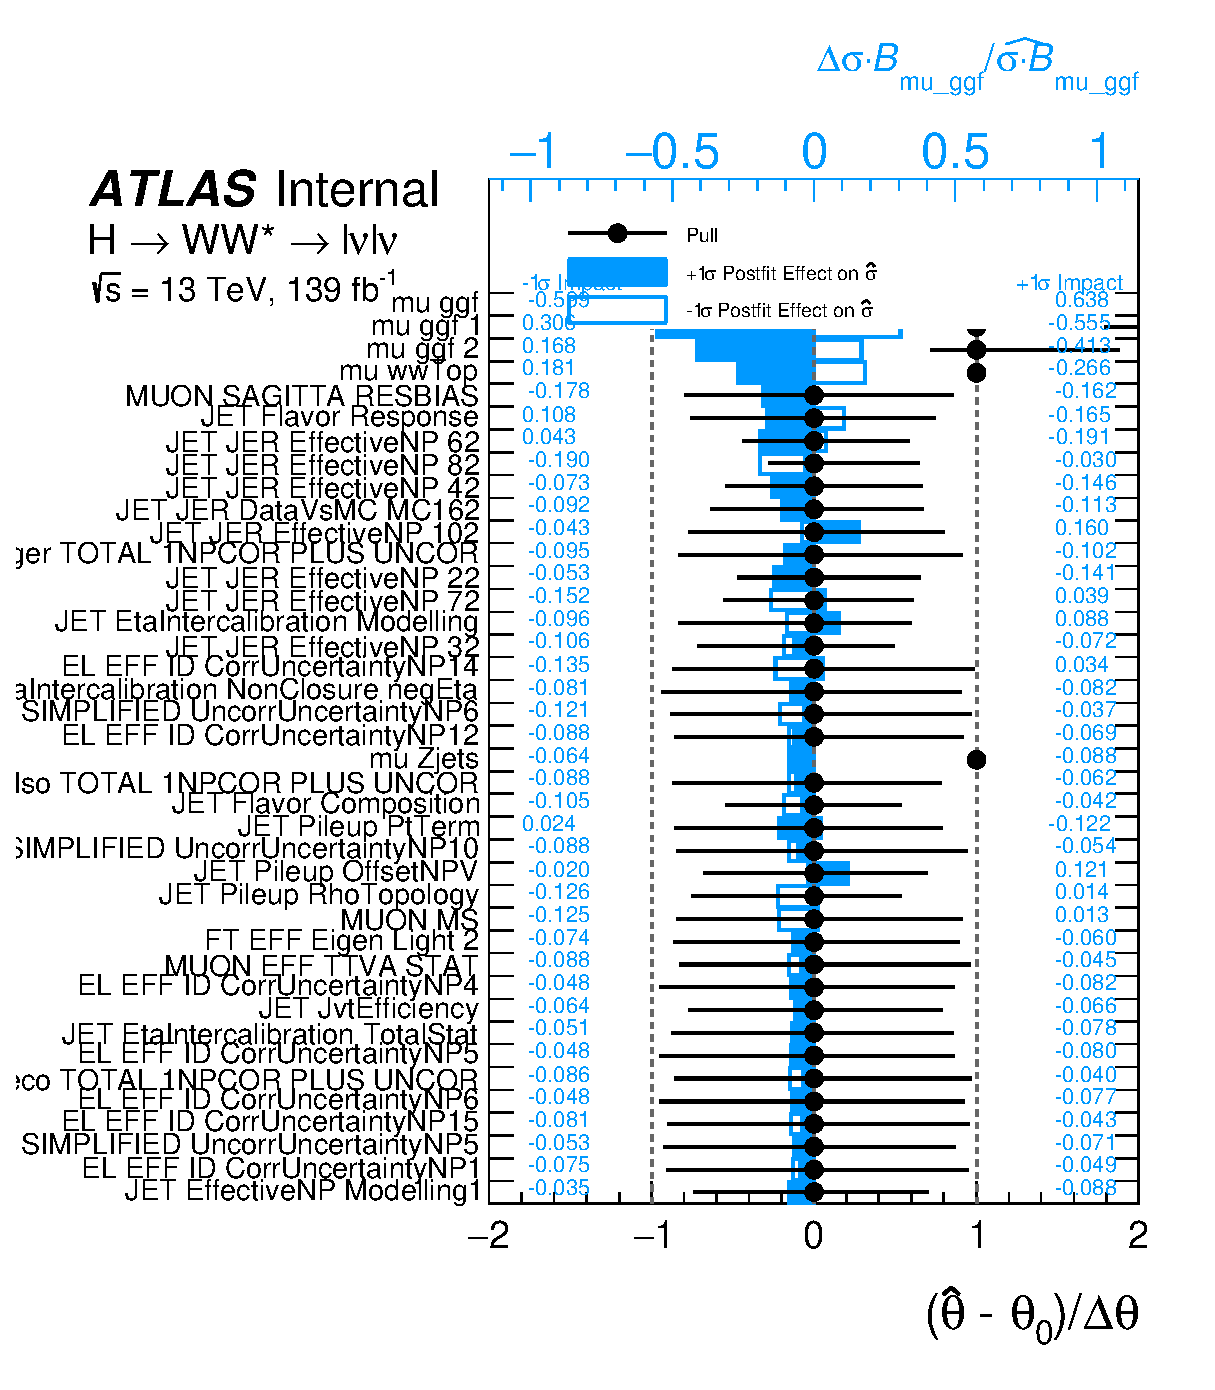
\includegraphics[width=0.3\textwidth]{Pictures/fitresults/impact_asimov_mu_ggf.eps}
%  }\hfill
%  \subfloat[$\mu_{\text{ggF1}}$]{
%      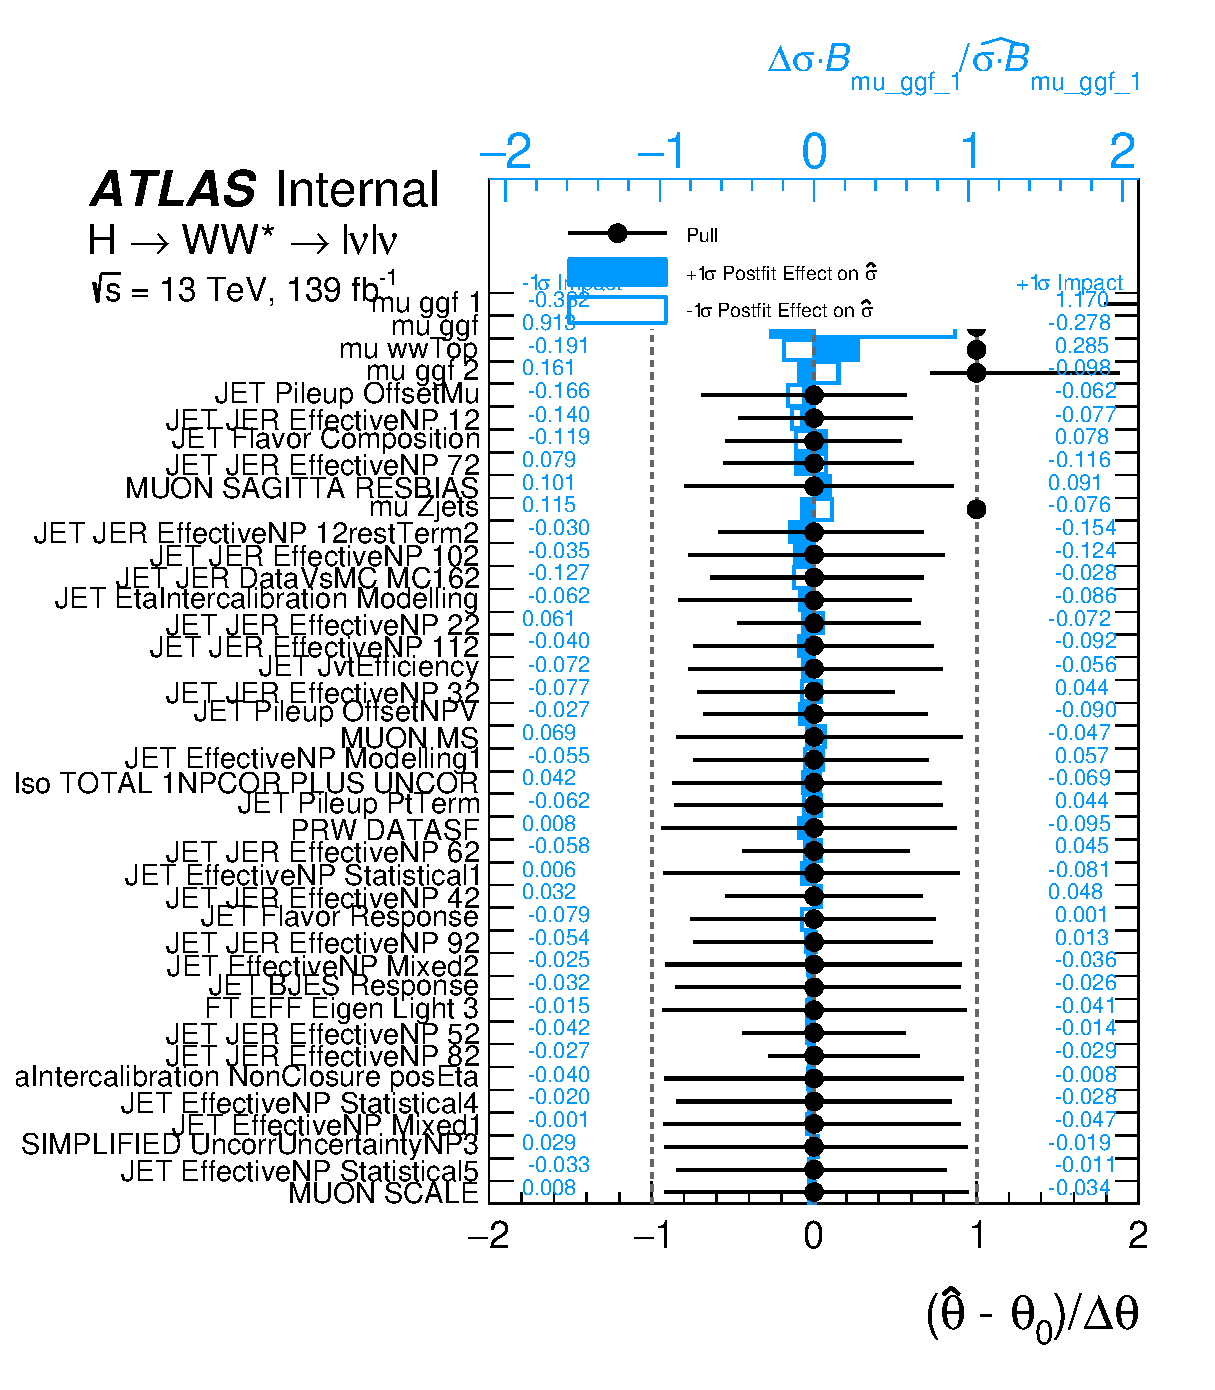
\includegraphics[width=0.3\textwidth]{Pictures/fitresults/impact_asimov_mu_ggf_1.eps}
%  }\hfill
%  \subfloat[$\mu_{\text{ggF2}}$]{
%      \includegraphics[width=0.3\textwidth]{Pictures/fitresults/impact_asimov_mu_ggf_2.eps}
%  }\hfill
%  \subfloat[$\mu_{\text{Top/}WW}$]{
%      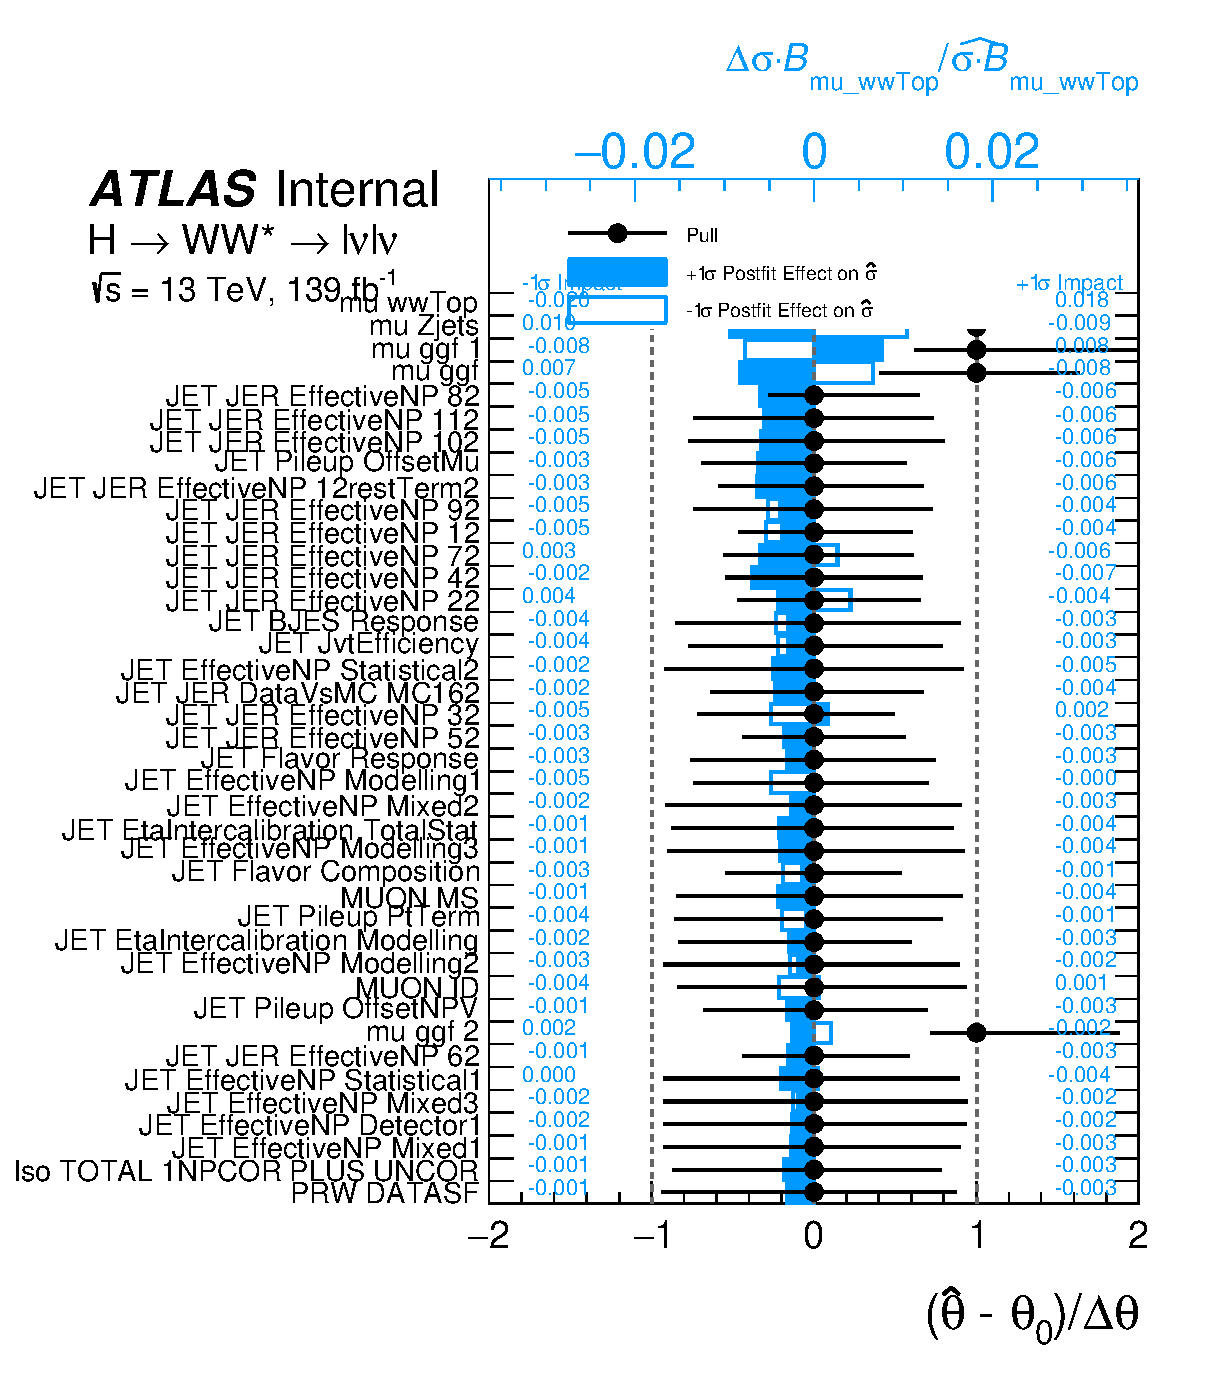
\includegraphics[width=0.3\textwidth]{Pictures/fitresults/impact_asimov_mu_wwTop.eps}
%  }\hfill
%  \subfloat[$\mu_{Z+\text{jets}}$]{
%      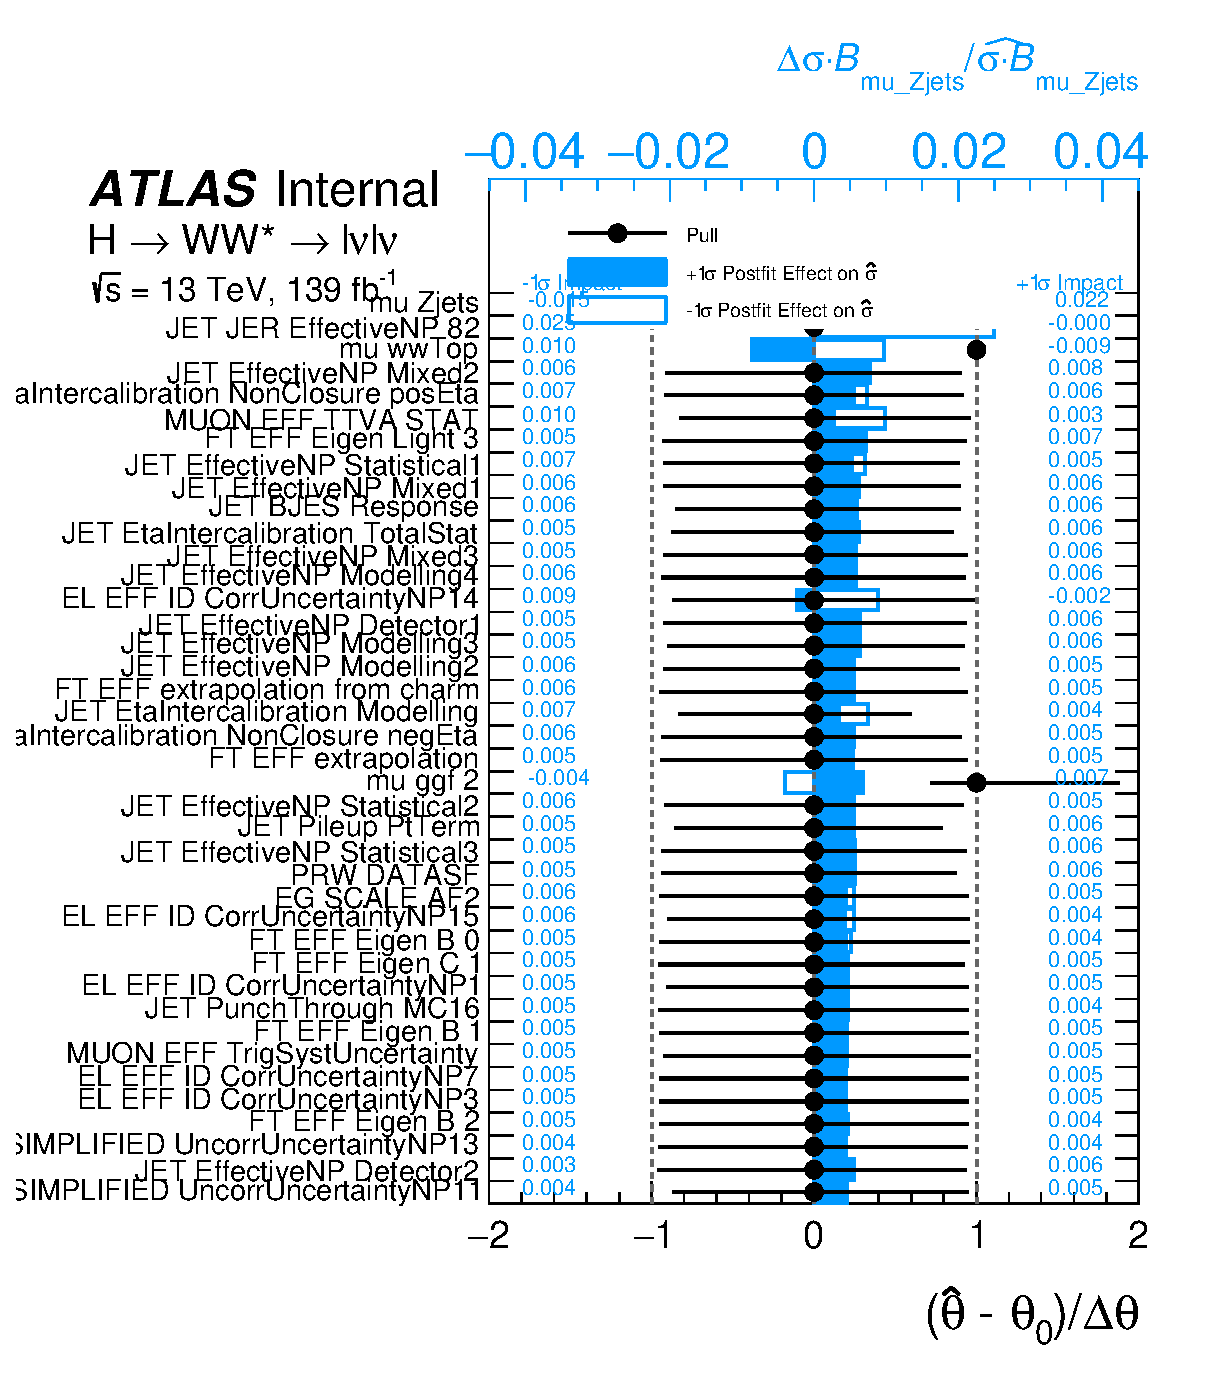
\includegraphics[width=0.3\textwidth]{Pictures/fitresults/impact_asimov_mu_Zjets.eps}
%  }%hfill
\caption{Post-fit effects of top 30 most impactful nuisance parameters on $\mu_{\text{VBF}}$ using the Asimov dataset.}
\label{fig:impactsasimov}
\end{figure}

We used the Asimov dataset to optimize fit strategies and selection criteria and to determine which uncertainies play large roles in this measurement. We have also suppressed the variations for which the MC statistical error is larger than the systematic. This is because some regions with very low statistics led to overconstraints on particular systematic uncertainties. The $Z+$jets and $WW$/top parameters have extremely high statistics in their control regions, so these contributions are dominated by their systematic errors. Figure~\ref{fig:impactsasimov} shows the expected effects of nuisance parameters in determining $\mu_{\text{VBF}}$. These effects are derived by changing each parameter individually by $\pm 1\sigma$ at the likelihood maximum. The measured effects of these changes are shown in blue in Figure~\ref{fig:impactsasimov} and ranked in order of total absolute impact. Notable uncertainties include those related to jet flavor composition, which plays a large role in rejecting dominant top background events, and uncertainties on jet pile-up, which cause potential errors in the jet kinematics. The impact of mis-identified leptons and the uncertainties associated with their fake factors, especially that regarding mis-identified lepton composition, is also significant.

\subsection{Observed results}
After examining and testing Asimov results, we unblind the analysis, or incorporate observed data in the statistical analysis\footnote{For this thesis, this is done privately without ATLAS collaboration approval. This result will be included in a forthcoming ATLAS publication.}. Fit parameters are measured by fitting simulated events with observed data and our overall results closely match those expected from the Asimov dataset. The signal strength for VBF Higgs is measured to be
\begin{equation}
\mu_{\text{obs}} = 1.04 ^{+0.20}_{-0.20} \text{ (Total) } ^{+0.17}_{-0.16} \text{(Stat.)} ^{+0.10}_{-0.10} \text{(Theor.)} ^{+0.04}_{-0.05} \text{(Exp.)},
\end{equation}
where contributions from experimental and theoretical systematics are  calculated just as in the Asimov dataset. These results closely match our expected Asimov values in terms of signal strength and uncertainty. This $\mu_\text{VBF}$ result confirms the hypothesis that signal VBF Higgs exist in the data within our signal region with a 6.6$\sigma$ signficance. This corresponds to a $p$-value of $2.0\times10^{-10}$ and is above the threshold for discovery. This observed $p$-value shows that the likelihood that the signal we observe is a statistical aberration is miniscule. The next section will describe how this result directly leads to the VBF fiducial cross section measurement. 

%Table~\ref{tab:datamuresults}. 

%\begin{table}[!h]
%  \begin{center}
%    \begin{tabular}{l|c|c|c|c|}
%        & \multicolumn{2}{|c|}{Fit value} & \multicolumn{2}{|c|}{Uncertainty} \\
%       Parameter & Stat-only & Stat+Sys & Stat-only & Stat+Sys \\
%      \hline
%       $\mu_{\text{VBF}}$ & 0.93 & 0.86 & 17.6$\%$ & 19.2$\%$ \\
%       $\mu_{\text{top/}WW}$ & 0.96 & 0.85 & 0.5$\%$ & 13$\%$ \\
%       $\mu_{\text{ggF-SR}}$ & 0.51 & 1.00 & 168.0$\%$ & 167$\%$ \\
%       $\mu_{\text{ggF1}}$ & 1.11 & 1.14 & 22.2$\%$ & 22.7$\%$ \\
%       $\mu_{\text{ggF2}}$ & 0.43 & 0.56 & 50.4$\%$ & 38.2$\%$ \\
%       $\mu_{\text{ggF3}}$ & 1.09 & 1.07 & 23.7$\%$ & 22.3$\%$ \\
%       $\mu_{Z+\text{jets}}$& 0.89 & 0.92 & 2.0 $\%$ & 16.7 $\%$ \\
%    \end{tabular}
%    \caption{Unblinded results for all floating parameters in stat-only and stat+systematic fits.}
%    \label{tab:datamuresults}
%  \end{center}
%\end{table}
%
%\begin{table}[!h]
%  \begin{center}
%    \begin{tabular}{l|c|c|c|}
%      Sample   & Pre-fit yield & Post-fit yield \\
%      \hline
%     VBF   &   166.1 & 29.5 \\
%      Top   &  368.9 & 1.5 \\
%      $WW$ & 192.12 & 2.4 \\
%      ggF &  21.5 & 36.5 \\
%      $Z+$jets & 281.7 & 6.4 \\
%      Fakes &  65.7 & -- \\
%      $V\gamma$ 23.5 & -- \\
%      $VH$ & 2.0 & -- \\
%      $ttH$ & 3.8 & -- \\
%      Total background & 960.2 &to add \\
%      Observed & 1125 & \\
%      \hline
%    \end{tabular}
%    \caption{Expected (pre-fit), predicted (post-fit) and observed event yields in the signal region. Uncertainties include statistical and systematic. }
%    \label{tab:sryields}
%  \end{center}
%\end{table}

Figure~\ref{fig:fitresultsregions} shows the expected and observed discriminant distributions in each of the signal and control regions included in the fit. Data (black) closely matches Standard Model simulations except for some individual bins where deviations are within the level of expected uncertainty. Data errors account for statistical uncertainties. 

\begin{figure}[!h]
\centering
  \subfloat[Signal region]{
      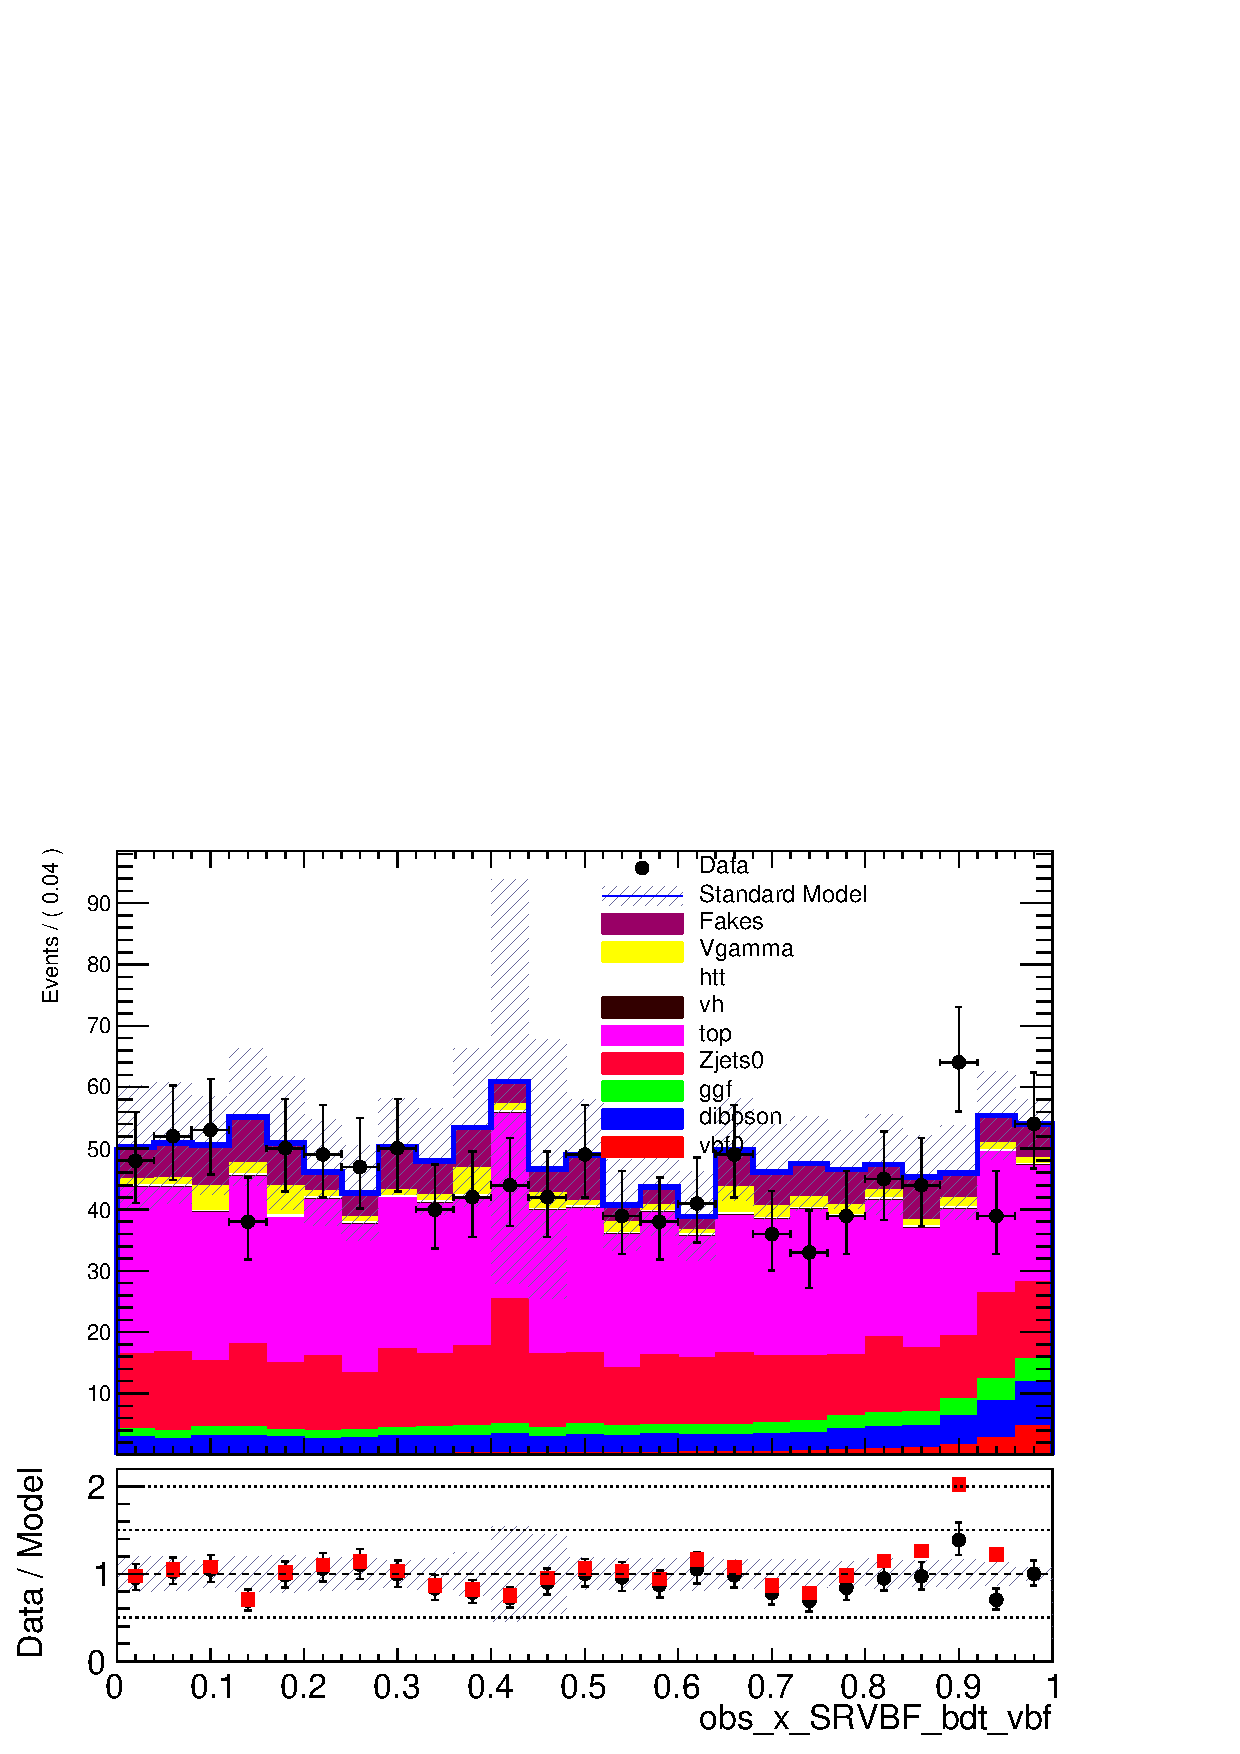
\includegraphics[width=0.3\textwidth]{Pictures/fitresults/SRVBF.pdf}
  }\hfill
  \subfloat[ggF SR control region]{
      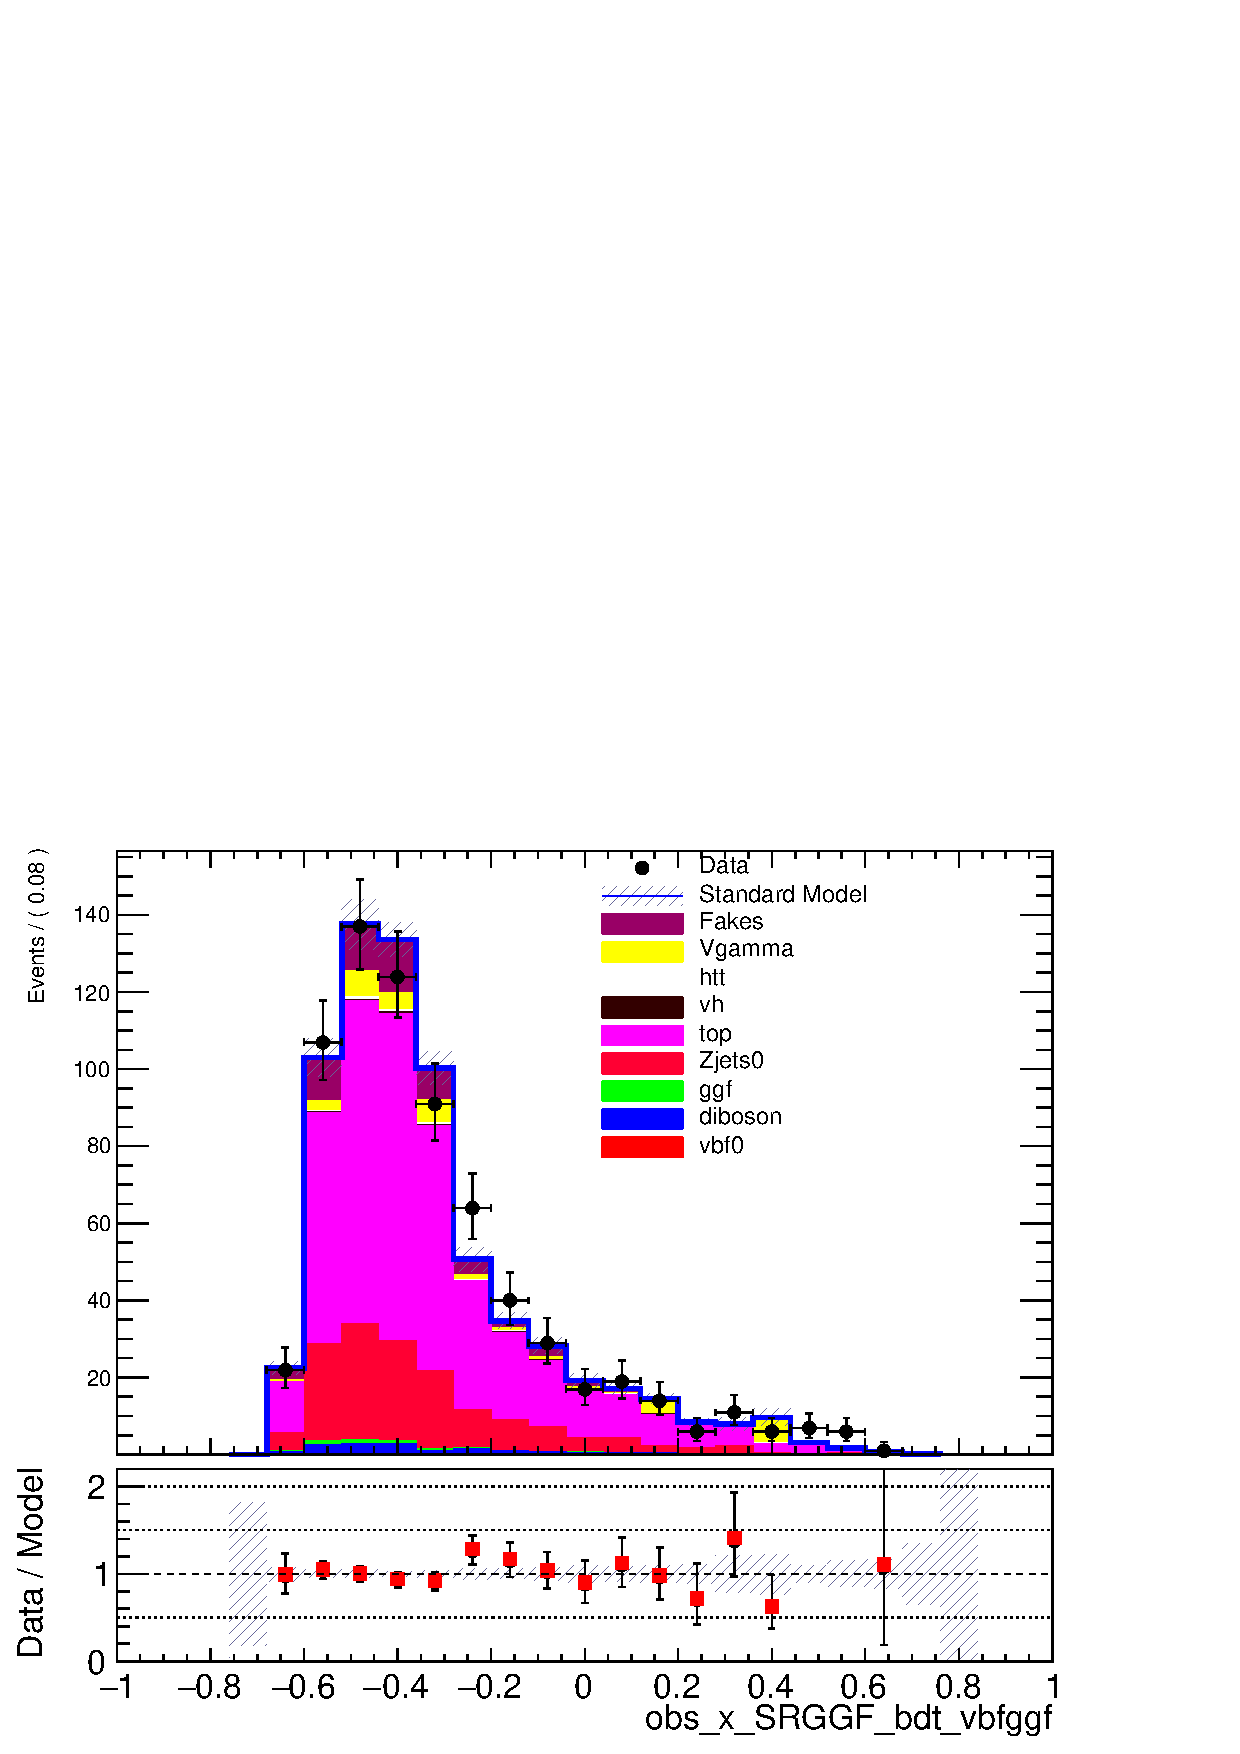
\includegraphics[width=0.3\textwidth]{Pictures/fitresults/SRGGF.pdf}
  }\hfill
  \subfloat[ggF 1 control region]{
      \includegraphics[width=0.3\textwidth]{Pictures/fitresults/CRGGF.pdf}
  }\hfill
  \subfloat[ggF 2 control region]{
      \includegraphics[width=0.3\textwidth]{Pictures/fitresults/CRGGF2.pdf}
  }\hfill
  \subfloat[ggF 3 control region]{
      \includegraphics[width=0.3\textwidth]{Pictures/fitresults/CRGGF3.pdf}
  }\hfill
  \subfloat[$Z+$jets control region]{
      \includegraphics[width=0.3\textwidth]{Pictures/fitresults/CRZjets.pdf}
  }\hfill
  \subfloat[Top/$WW$ control region]{
      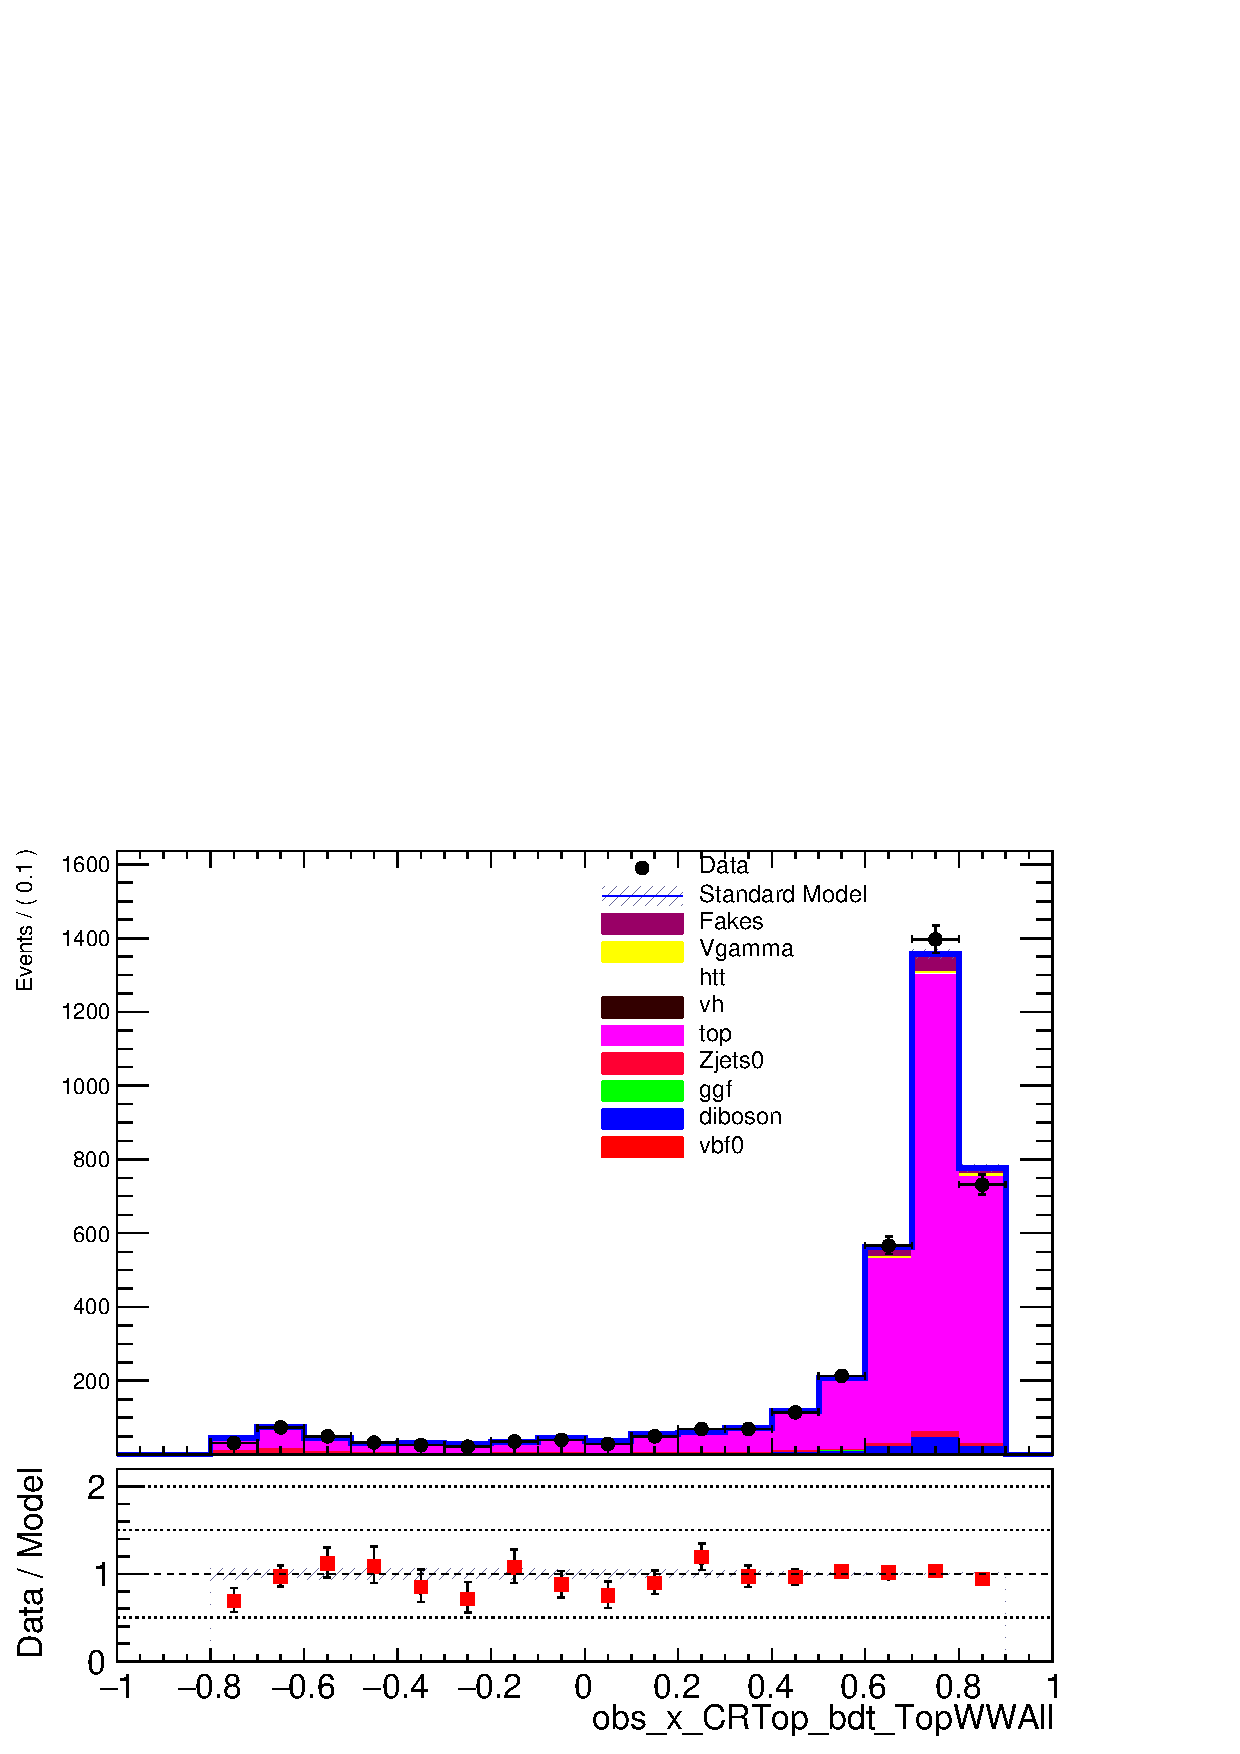
\includegraphics[width=0.3\textwidth]{Pictures/fitresults/CRTop.pdf}
  }%hfill
{\caption{Binned distributions for each signal and control region shown after stat+sys fit where ratio between data and MC predictions is shown (black). Error bands show statistical uncertainties.}
\label{fig:fitresultsregions}}
\end{figure}

Figure~\ref{fig:correlations} shows correlations between floating parameters in the fit using a stat-only scheme where only the seven floating signal strength parameters are included. This is to focus on the parameters which most impact the fit, although we also inspect correlations between our nuisance parameters. This is included in Ref.~\cite{ourSupportNote}. Correlations between fit parameters would indicate potential instability in the overall result as small changes in some estimated parameters would severely impact others. The correlation between measured background and signal parameters is small, through some parameters like $\mu_{ggF1}$ and $\mu_{ggF3}$ are anti-correlated. We have further tested the robustness of these parameters by changing their binning and discriminants and concluding that our overall Asimov fit result remains stable.  

\begin{figure}[!h]
\centering
\includegraphics[width=0.75\textwidth]{Pictures/fitresults/correlation_stat.eps}
\caption{Correlations between floating parameters after a stat-only fit.}
\label{fig:correlations}
\end{figure}

We visualize our likelihood minimization in Figure~\ref{fig:scan}. We perform a one-dimensional scan of our parameter of interest, $\mu_{\text{VBF}}$, using the inputs and distributions of our fit. The figure shows fit results for $\mu_{\text{VBF}}$ if we use all systematics or only statistical uncertainties. These results demonstrate that the statistical uncertainties are dominant in determining our final fit value. The stat-only analysis has an expected uncertainty of $^{+17.0\%}_{-16.3\%}$ while including all systematics gives an expected $^{21.0\%}_{-18.8\%}$. Observed results are very similar. Our observed signal significance is $1.04$ with total uncertainties of $^{20.3\%}_{-19.9\%}$ closely matching our expectation. Expected results are derived using Asimov data and shown in red while observed results using data are displayed in black. The observed and expected results are in agreement, confirming our expectations. We can split our systematic contributions into theoretical and experimental components by fixing each type of systematic to a constant value within the fit. Figure ~\ref{fig:scan2} shows the results of the fit on signal significance removing experimental and theoretical uncertainties, respectively. In both cases statistical uncertainties are the leading source of error, but beyond that we can see contributions from theoretical uncertainties surpass those from experimental uncertainties.  

\begin{figure}[!h]
\centering
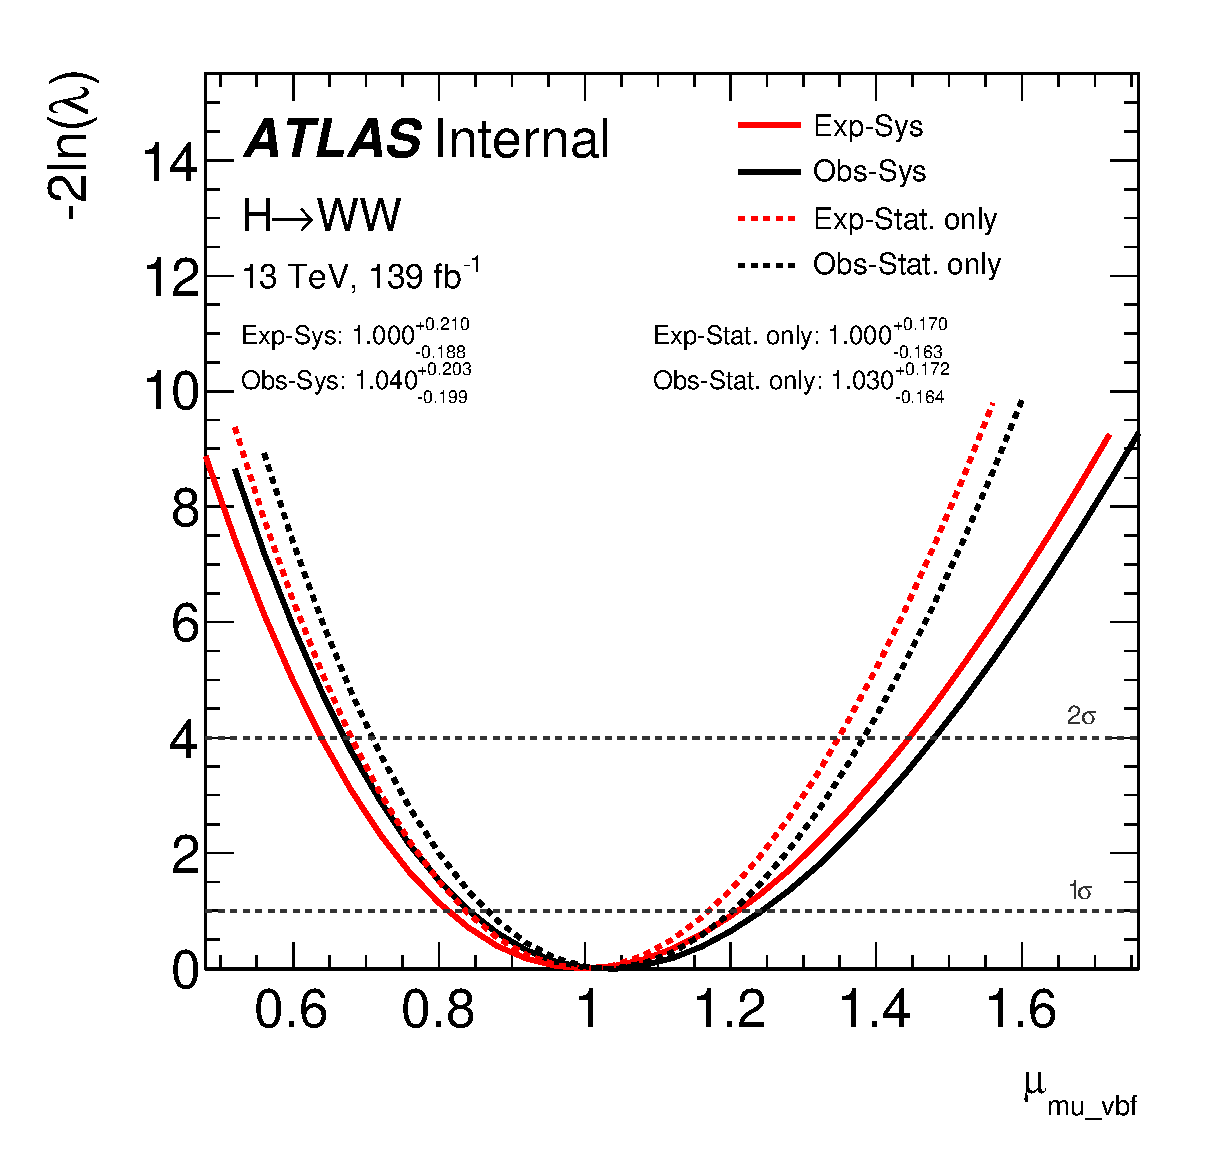
\includegraphics[width=0.7\textwidth]{Pictures/fitresults/mu_vbf_stattotal.eps}
\caption{Scan of $\mu_{\text{VBF}}$ negative log-likelihood using observed data (black) and Asimov expected results (red) and demonstrating the results using all systematics and only statistical uncertainties.}
\label{fig:scan}
\end{figure}

\begin{figure}[!h]
\centering
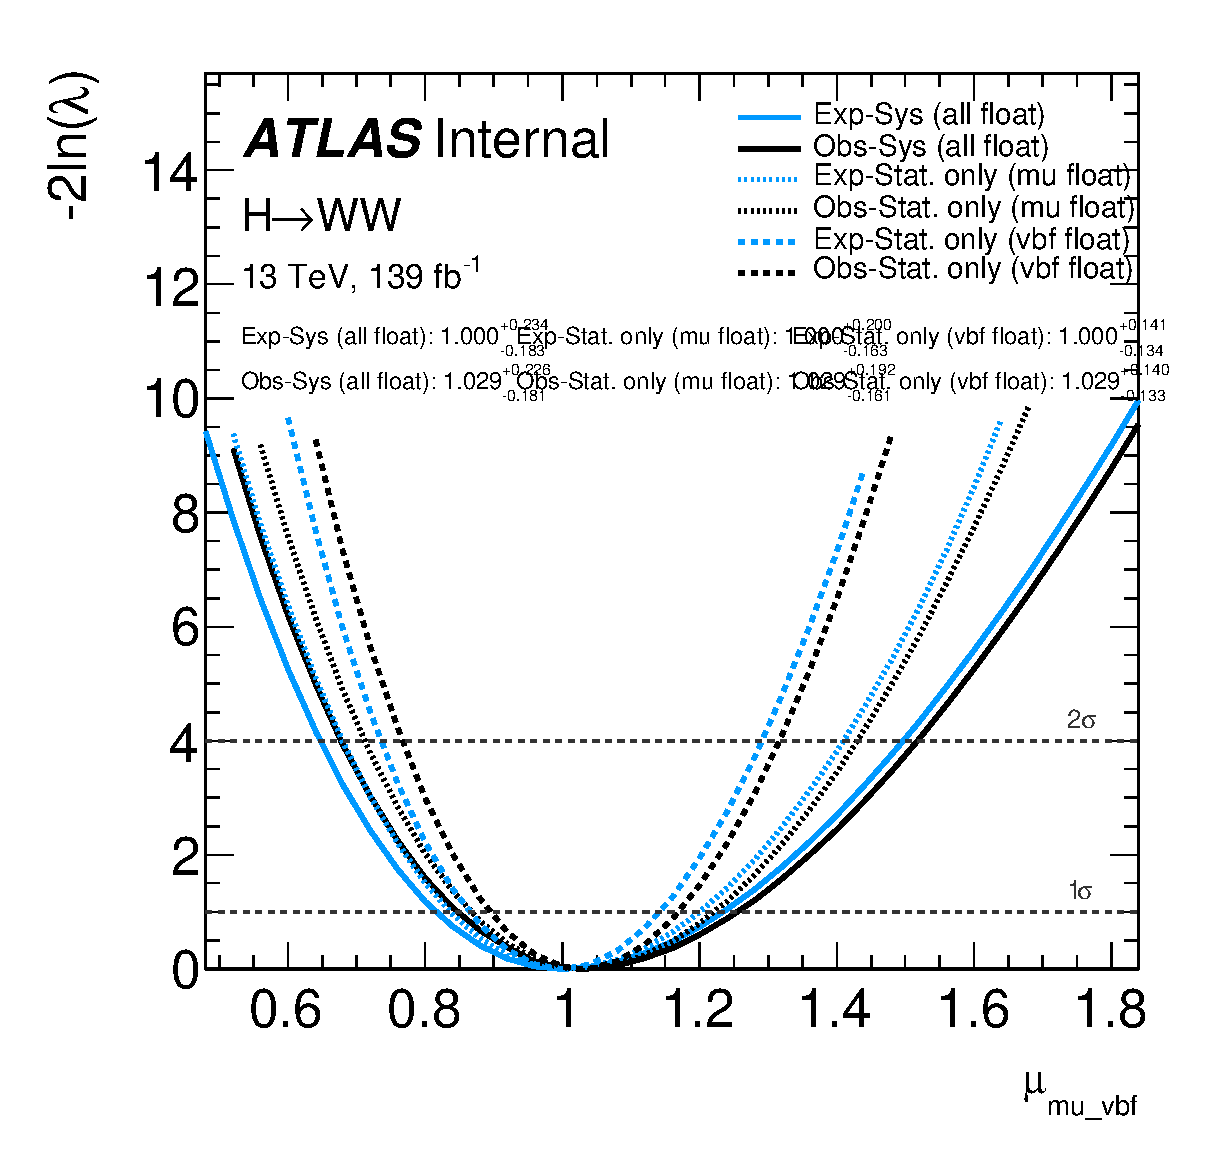
\includegraphics[width=0.7\textwidth]{Pictures/fitresults/mu_vbf.eps}
\caption{Scan of $\mu_{\text{VBF}}$ negative log-likelihood using observed data (black) and Asimov expected results (blue) and demonstrating the results using all statistical and theoretical uncertainties and theoretical and experimental uncertainties.}
\label{fig:scan2}
\end{figure}

\begin{figure}[!h]
\centering
%  \subfloat[$\mu_{\text{VBF}}$]{
      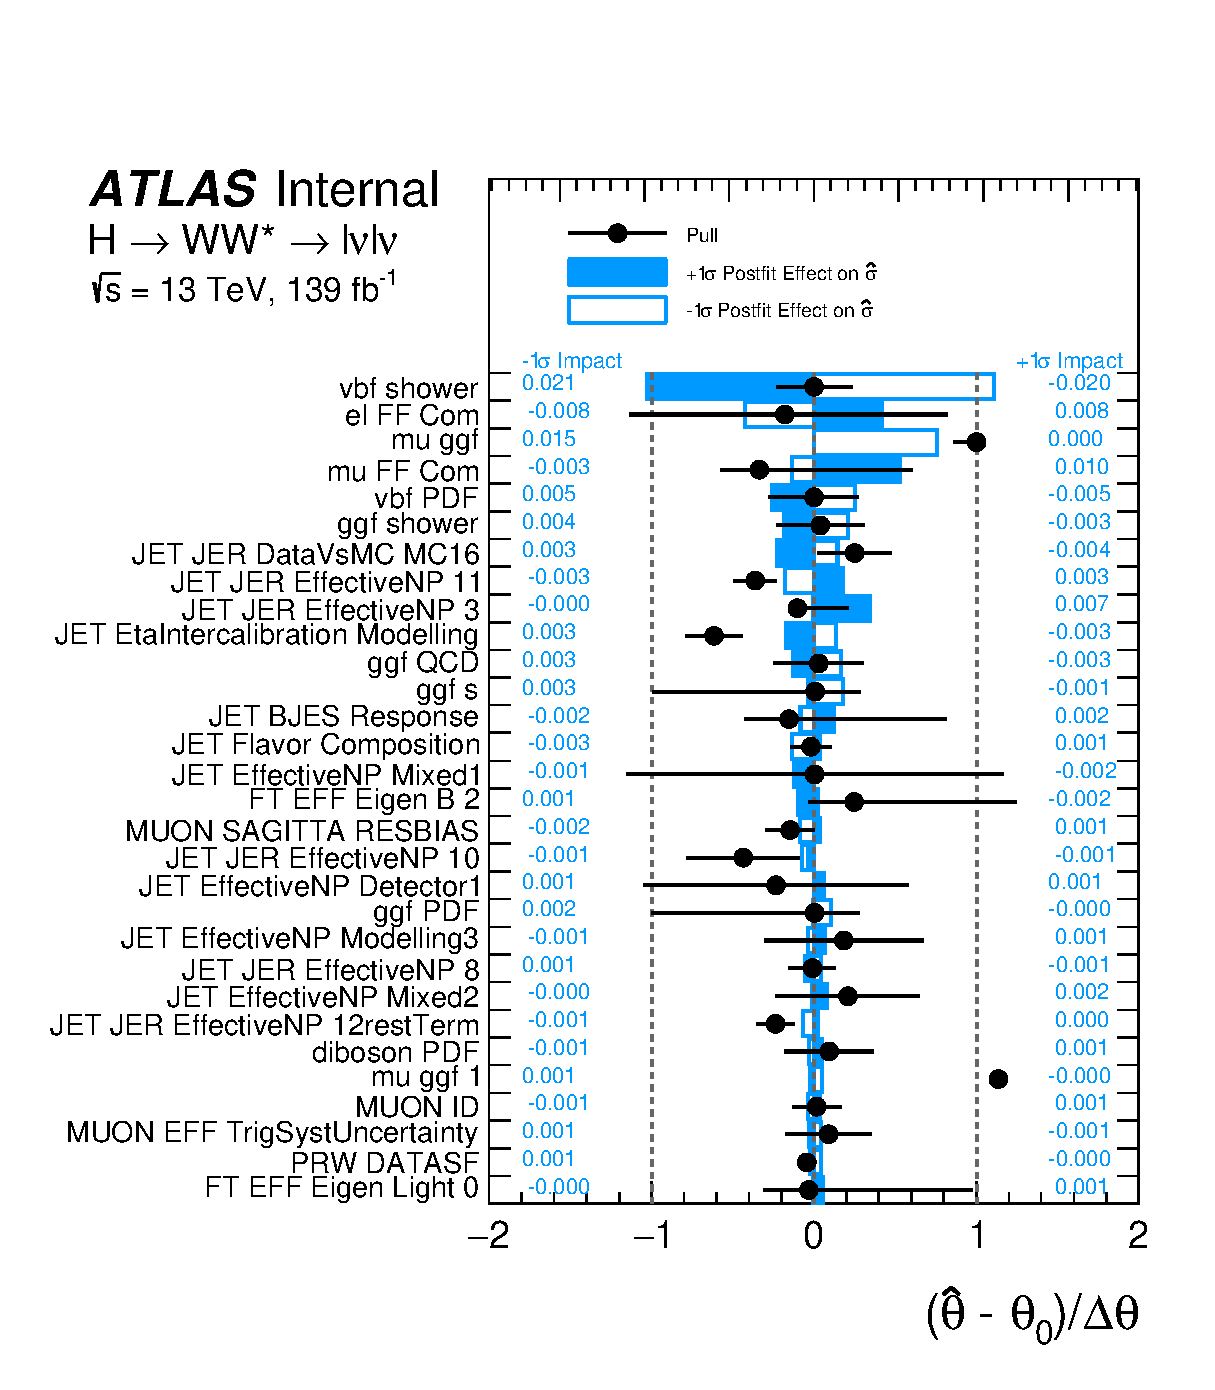
\includegraphics[width=0.6\textwidth]{Pictures/fitresults/impact_data_mu_vbf.eps}
%  }\hfill
%  \subfloat[$\mu_{\text{ggF}}$]{
%      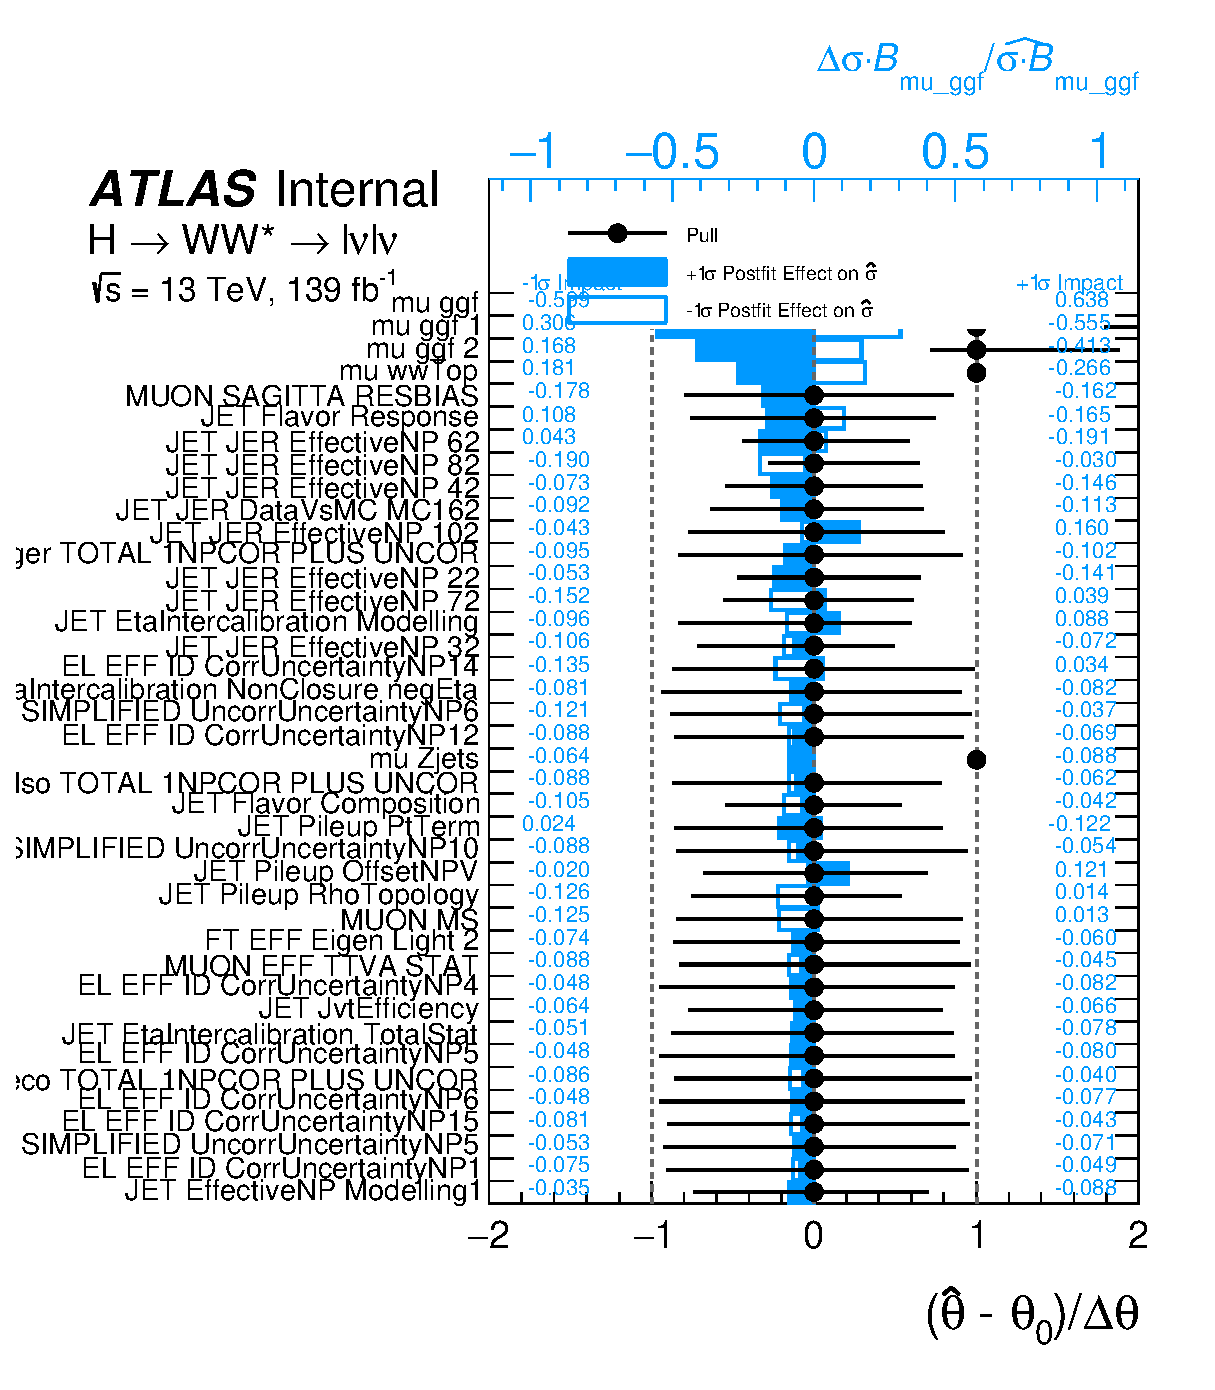
\includegraphics[width=0.3\textwidth]{Pictures/fitresults/impact_asimov_mu_ggf.eps}
%  }\hfill
%  \subfloat[$\mu_{\text{ggF1}}$]{
%      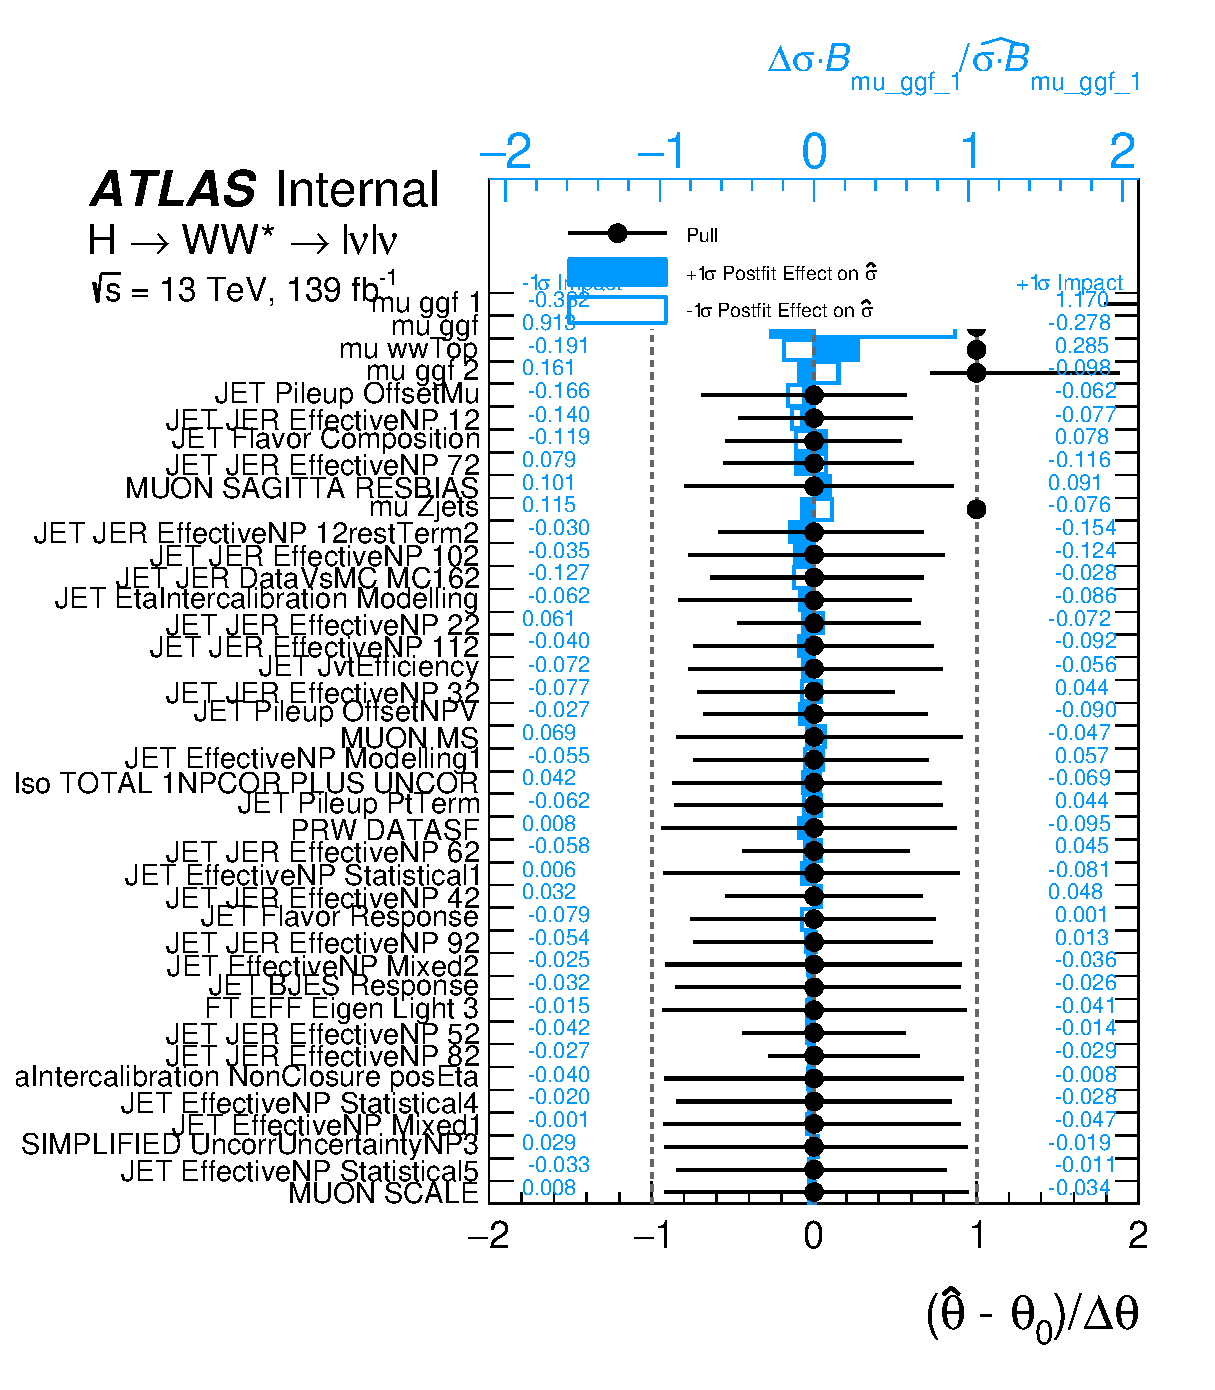
\includegraphics[width=0.3\textwidth]{Pictures/fitresults/impact_asimov_mu_ggf_1.eps}
%  }\hfill
%  \subfloat[$\mu_{\text{ggF2}}$]{
%      \includegraphics[width=0.3\textwidth]{Pictures/fitresults/impact_asimov_mu_ggf_2.eps}
%  }\hfill
%  \subfloat[$\mu_{\text{Top/}WW}$]{
%      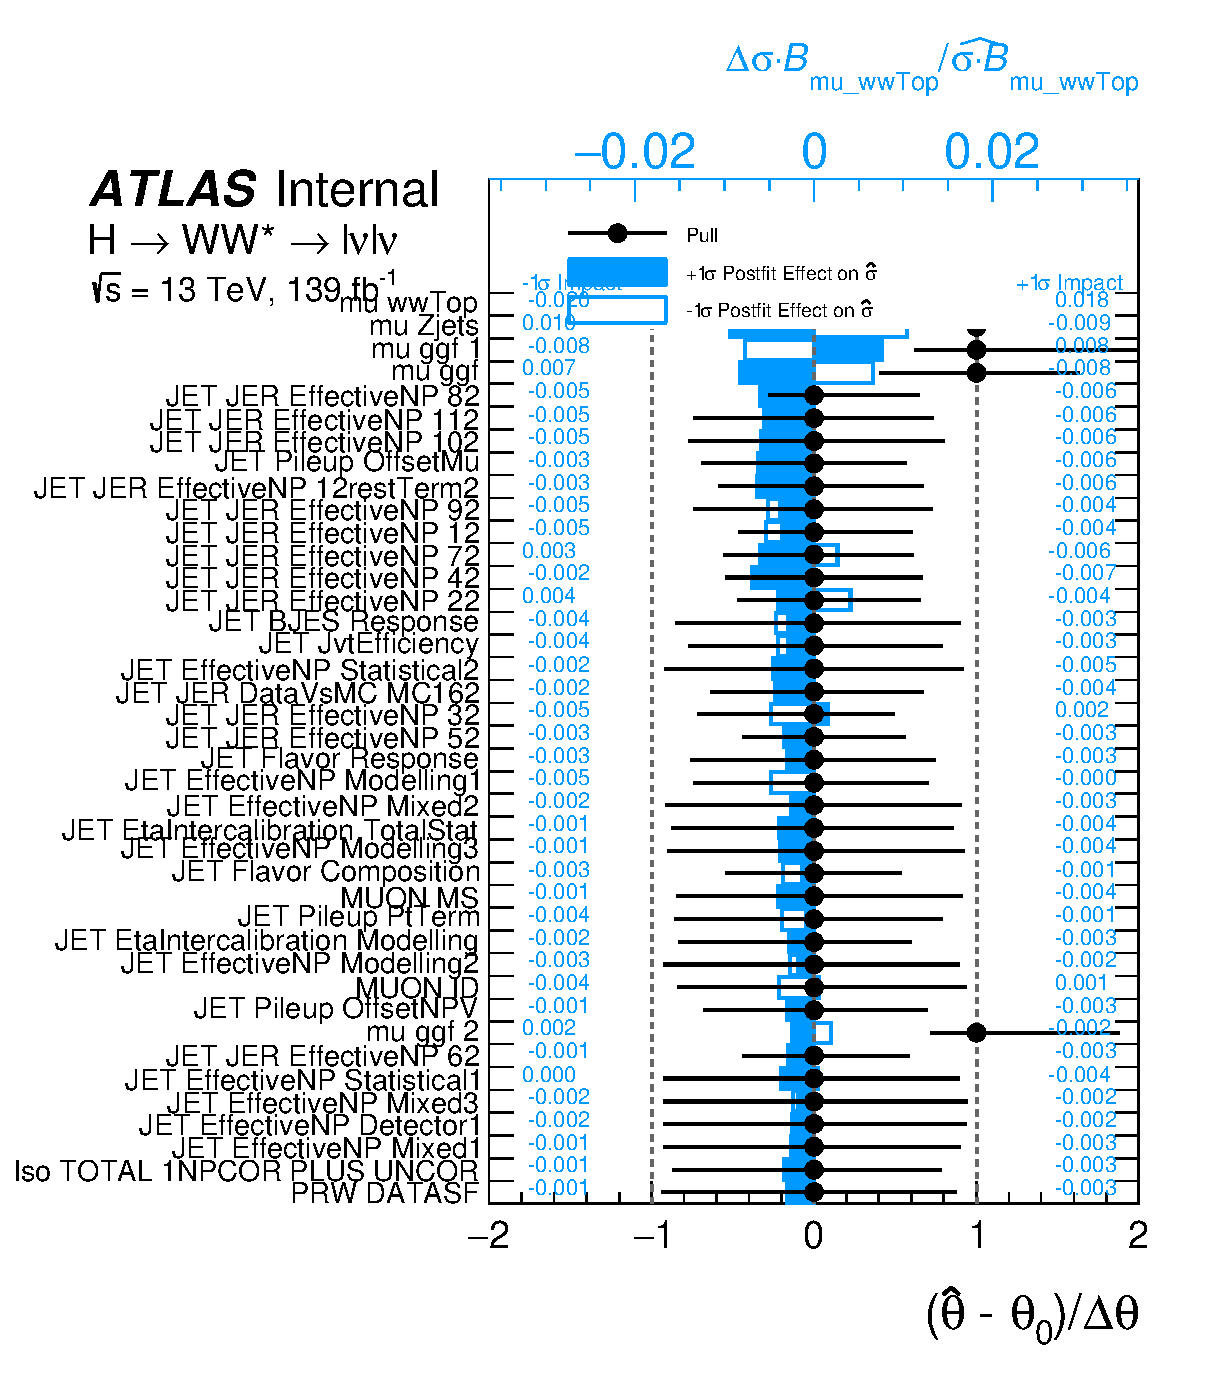
\includegraphics[width=0.3\textwidth]{Pictures/fitresults/impact_asimov_mu_wwTop.eps}
%  }\hfill
%  \subfloat[$\mu_{Z+\text{jets}}$]{
%      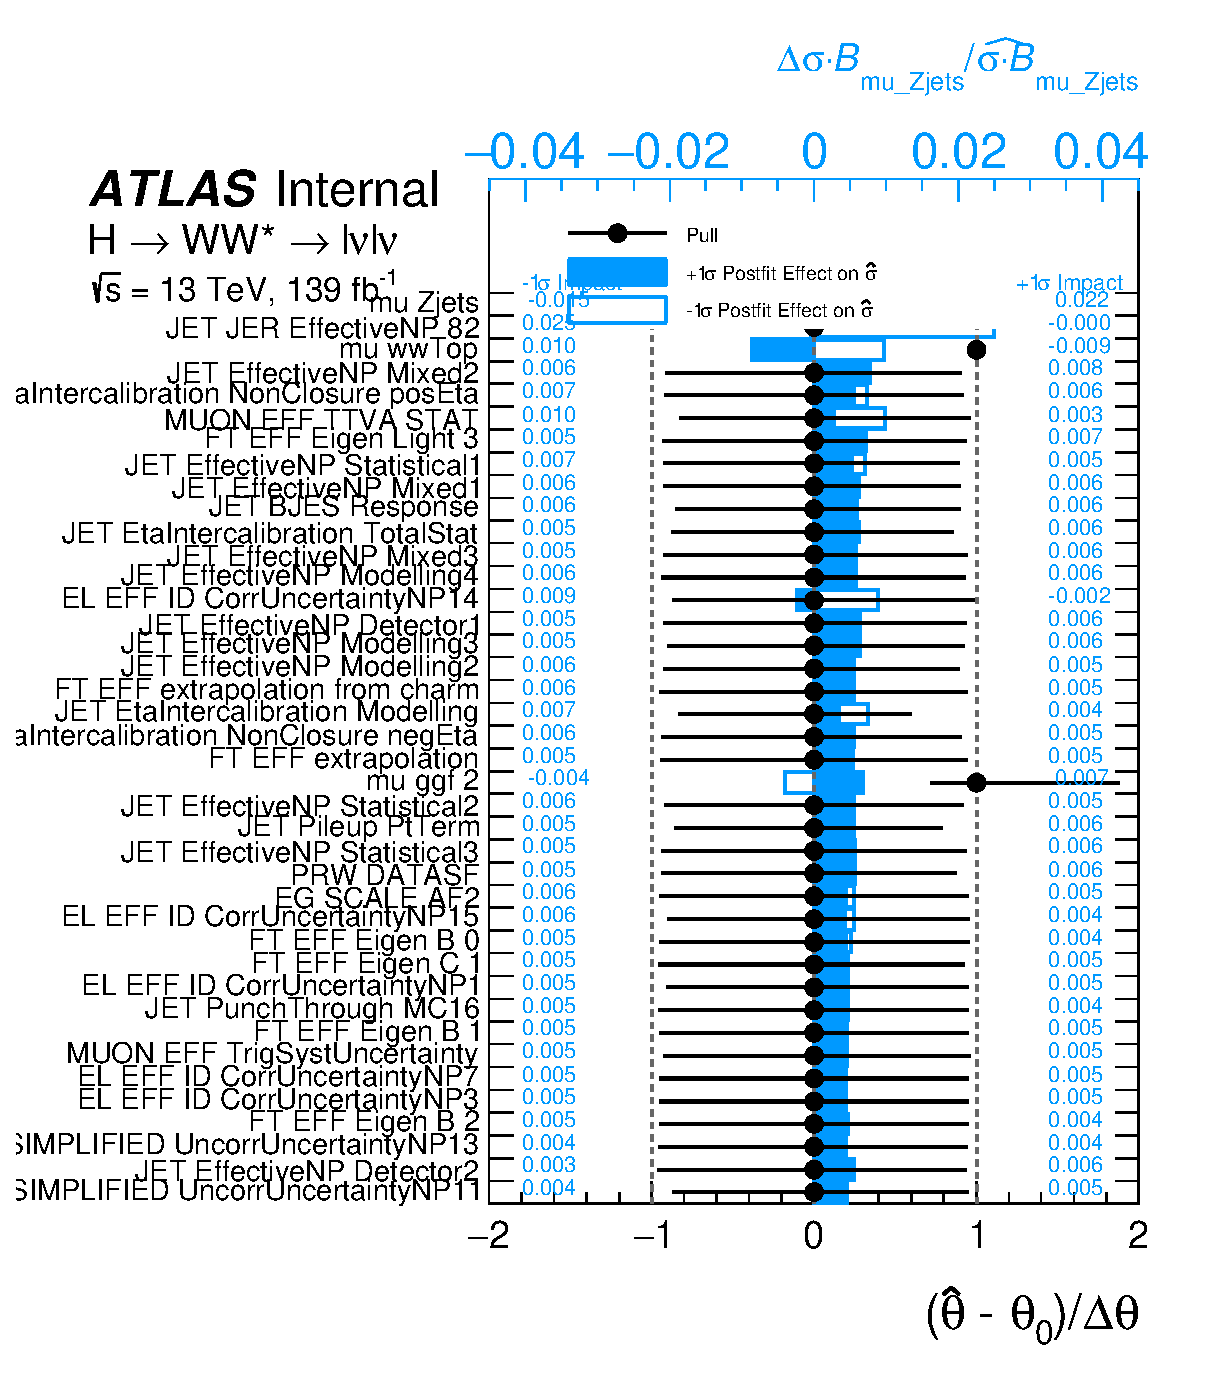
\includegraphics[width=0.3\textwidth]{Pictures/fitresults/impact_asimov_mu_Zjets.eps}
%  }%hfill
{\caption{Post-fit effects of top 30 most impactful nuisance parameters on $\mu_{\text{VBF}}$ using observed dataset.}
\label{fig:impacts}}
\end{figure}

Figure~\ref{fig:impacts} shows the 30 largest contributors to the error on the measurement of the VBF parameter for the measured signal strength. As in the Asimov case, these effects are derived by changing each parameter individually by $\pm 1\sigma$ at the likelihood maximum and ranked in order of total absolute impact.

While ggF is not the largest background in the signal region, its similar signature to VBF Higgs production makes it particularly difficult to differentiate from our signal. The combined $WW$/top estimation has a similarly large effect on the measurement. The backgrounds are easily differentiated from the signal but outsize the VBF Higgs by far, even in the signal region. Jet-related experimental systematics have the largest effects of any, with impacts from jet energy resolution, jet pile up, and jet flavor tagging. This is expected because of the large range of jet kinematic variables in our multivariate analysis. Finally, theory systematics are pivotal to the overall estimation. VBF and ggF theory uncertainties are dominant---particularly VBF shower and PDF and ggF shower parameters. Chapter 5 describes the size of these variations and explains their role in the final measurement. All theoretical systematics in this analysis are estimated using floating global variations. This intentionally overestimates the uncertainties since the final analysis will contain shape systematics that are not accounted for with this method. One of the largest overestimates comes from the diboson PDF theory parameter. Since this background is estimated within the signal region, its yield is normalized there, therefore shape systematics will have the primary effect. Chapter 5 shows that these shape variations are small, thus we can expect that the $WW$ PDF uncertainty will have a smaller effect when shape systematics are included. 

The fit results shown in this thesis demonstrate the most recent calculations and developments from the VBF $H\rightarrow WW$ fiducial cross-section measurement. These fit results produce event yields for each of our measured parameters which are then used to extract VBF Higgs fiducial and inclusive cross section measurements.

\section{Fiducial and inclusive cross sections}
This analysis aims to measure the total VBF $H\rightarrow WW^*\rightarrow\ell\nu\ell\nu$ cross-section in both a particular fiducial region and in a more inclusive region. Our analysis group also has the goal of measuring fiducial differential $H\rightarrow WW^*$ cross-sections over a range of kinematic variables, though these measurements are beyond the scope of this thesis. In each case, the measurement must be translated from one that only represents conditions in the ATLAS detector to values that can be understood with a broad range of theoretical models. For fiducial measurements, this can be done relatively simply with a $C$ factor, which accounts for  detector effects that would lower the overall cross section, like detector inefficiences and resolution effects. The fiducial region is defined so that it is applicable to both reconstructed and purely theoretical, called truth level, events. This fiducial region defines the conditions under which the cross-section is measured. The fiducial cross-section is defined as
\begin{equation}
\sigma_{\text{VBF}H\rightarrow WW^*\rightarrow\ell\nu\ell\nu}^{\text{fid}} = \frac{N_{\text{obs}}-N_{\text{bkg}}}{C\times\mathcal{L}},
\end{equation} 
where $\mathcal{L}$ is the integrated luminosity and $N_{\text{obs}}$/$N_{\text{bkg}}$ is the observed and estimated background number of events, respectively. $N_{\text{bkg}}$ is calculated through the simultaneous fit with simulated and observed events. The fiducial phase space is defined as close to the reconstruction-level signal region as possible to minimize theoretical extrapolation. Table~\ref{tab:fiducial} lists all fiducial cuts that describe the phase space. These include geometric requirements on lepton number, flavor, sign, and kinematics, missing energy, jet number, as well as other VBF specific requirements (OLV and CJV cuts). 
%Fiducial Volume
\begin{table}[!ht]
\centering
\begin{tabular}{|c|}
\hline
Fiducial Requirement \\
\hline
$|\eta(\ell)|<2.5$ \\
$p_T^{\text{lead}}>22$GeV \\
$p_T^{\text{sublead}}>15$GeV \\
$N_{\text{leptons}}\geq2$ \\
Leptons required to be opposite flavor and sign \\
$\Delta R(\ell,\ell) >$0.1 \\
$m_{\ell\ell}>10$GeV \\
$E_T^{\text{miss}}>$20GeV \\
$p_T$(jet)$>$30 GeV \\
$|\eta\text{(jet)}|<4.5$ \\ 
$N_{\text{jets}} \geq 2$ \\
$N_{b\text{-jet}} < 1$ \\
$m_{jj} >200$GeV \\
$\Delta Y_{jj}>2.1$ \\
$\Delta R(\ell,\text{jet})>0.4$ \\
OLV$=1$ \\
CJV$>20$GeV \\
\hline
\end{tabular}
\caption{Fiducial phase space definition}
\label{tab:fiducial}
\end{table}
These cuts represent the space within which both reconstruction-level and truth-level cross-sections are measured. Yields are extracted from the statistical fit and a $C$-factor is defined, 
\begin{equation}
C = \frac{N_\text{fid}}{N_{\text{reco}}},
\end{equation}
where $N_\text{fid}$ is extacted from theoretical simulation. Powheg$+$Pythia8 are used to extract theoretical yields in the fiducial region. The truth-level cutflow is shown in Table~\ref{tab:truth}. There are $371.5\pm0.6$ truth level VBF Higgs events in the final fiducial region, thus $C=2.23\pm 0.40$. The uncertainties on $C$ are dominated completely by the uncertainty on $N_{\text{reco}}$, which is extracted from the liklihood maximization.  

\begin{table}[!ht]
\centering
\begin{tabular}{c||c}
\textbf{Full Run 2} & \textbf{Powheg$+$Pythia8 VBF} \\
\hline
$|\eta(\ell)|<2.5$ & 144 \\
$p_T^{\text{lead}}>22$GeV &144 \\
$p_T^{\text{sublead}}>15$GeV & 144\\
OS Leptons & 1414 \\
$\Delta R(\ell,\ell) >$0.1 & 1345 \\
$m_{\ell\ell}>10$GeV & 1345  \\
$N_{\text{jets}}\geq2$ & 744\\
$m_{jj} \geq 200$ GeV & 638  \\
$\Delta Y_{jj}>2.1$ & 612  \\
$E_{\text{T}}^{miss}>20$ GeV & 545  \\
CJV$>20$ GeV & 483 \\
OLV bool & 446  \\
$b$-veto & 437  \\
$Z\rightarrow\tau\tau$ veto & 371 \\
\hline
\end{tabular}
\caption{Cutflow showing VBF Higgs events generated with Powheg$+$Pythia8 at truth-level with all fiducial selection requirements~\cite{ourSupportNote}. }
\label{tab:truth}
\end{table}

Using this value for $C$ and a predicted cross section value of 2.67~fb, from the Powheg$+$Pythia8 fiducial cross-section truth estimate, we find a final cross-section measurement of:
\begin{equation}
\sigma_{\text{fid,obs}} = 2.78^{+0.56}_{-0.53} \text{ fb} 
\end{equation}

This measured value closely matches our expected truth value, well within one standard deviation, and its error of $\approx20\%$ is well below the previous $\approx50\%$ uncertainty measured on the $H\rightarrow WW^*$ VBF production cross section with 36.1 fb$^{-1}$~\cite{Aaboud_2019}. 
%This standard deviation corresponds to a 6$\sigma$ observation with $p= $. The VBF $H\rightarrow\ell\nu\ell\nu$ cross-section is observed with a 1/100000 chance of statistical anomaly.  

The inclusive cross-section requires one additional acceptance correction factor, $A$, which is estimated from theoretical calculations and extrapolates the fiducial cross section to a more inclusive phase space defined solely by a requirement for $N_{\text{jets}}\geq2$, where each jet has $p_T>30$~GeV. This will be calculated from
\begin{equation}
\sigma_{VBF}^{\text{incl}} = \frac{\sigma_{VBF}^{\text{fid}}}{A}.
\end{equation}
The inclusive cross-section widens the applicable phase space of the measurement and provides another useful metric to compare data with expected Standard Model results. The $A$ factor is found through theoretical calculations which use Powheg to estimate VBF processes at next-to-leading order in QCD and inclusive cross-section calculations from the Yellow Report \cite{LHCCrossSectionWG}. Using the events in Table~\ref{tab:truth}, the theoretical fiducial cross section is found to be $2.67$~fb and the inclusive VBF $H\rightarrow WW^*\rightarrow \ell\nu\ell\nu$ cross section is calculated at 85.8$\pm 3.1$~fb. The inclusive cross section is calculated with the VBF $H$ cross-section derived for $\sqrt{s}=13$ TeV and $m_H=125$ GeV, and the branching fractions for $H\rightarrow WW^*$ and $WW^*\rightarrow\ell\nu\ell\nu$.  The acceptance factor is measured to be $0.031 \pm 0.006$. Using this factor, we measure an inclusive cross-section of
\begin{equation}
\sigma_{\text{incl,obs}} = 89.2^{+18.3}_{-17.3} \text{ (Total) } ^{+15.4}_{-14.8} \text{ (Stat.) } ^{+9.5}_{-9.5} \text{ (Theor.) } ^{+4.8}_{-4.8} \text{ (Exp.)} \text{ fb}.
\end{equation} 
This value again matches our expected Standard Model inclusive cross section within one standard deviation and provides high precision on the VBF $H\rightarrow WW^*\rightarrow\ell\nu\ell\nu$ inclusive cross section. Statistical uncertainties are dominant in this measurement, but theoretical uncertainties, including those described in the Yellow Report, also play a leading role in the total precision of the measurement.   
